\documentclass[12pt,letterpaper]{article}  % letterpaper is US standard (8.5" x 11")

% essential packages
\usepackage[utf8]{inputenc}
\usepackage[T1]{fontenc}
\usepackage{amsmath}
\usepackage{amsfonts}
\usepackage{amssymb}
\usepackage{amsthm}
\usepackage{graphicx}
\graphicspath{{../../results/figures/manuscript/}}
\usepackage{hyperref}
\usepackage{geometry}
\usepackage{setspace}
\usepackage{xcolor}
\usepackage{enumitem}
\usepackage{parskip}  % Removes paragraph indentation and adds space between paragraphs
\usepackage{float}
\usepackage{subcaption}
\usepackage{authblk}  % For author affiliations
\usepackage{natbib}  % For bibliography management

% page layout
\geometry{
    letterpaper,  % Options include:
    % letterpaper (8.5" x 11")
    % legalpaper (8.5" x 14")
    % a4paper (210mm x 297mm)
    % a5paper (148mm x 210mm)
    % b5paper (176mm x 250mm)
    % executive (7.25" x 10.5")
    margin=2cm }

% custom styling
\definecolor{linkcolor}{RGB}{0, 90, 160}
\hypersetup{
    colorlinks=true, linkcolor=linkcolor, urlcolor=linkcolor, citecolor=linkcolor }

% custom commands
\newcommand{\E}{\mathbb{E}}
\renewcommand{\P}{\mathbb{P}}
\newcommand{\V}{\text{Var}}

% theorem environments
\theoremstyle{definition}
\newtheorem{definition}{Definition}
\newtheorem{theorem}{Theorem}
\newtheorem{lemma}{Lemma}
\newtheorem{proposition}{Proposition}
\newtheorem{corollary}{Corollary}
\newtheorem{remark}{Remark}

% document info
\title{Conditional Extreme-Path Benchmarks for Sequential Probability Forecasts}
\author{Jonathan Pipping-Gam\'on \& Abraham J. Wyner\\
{\small Department of Statistics, University of Pennsylvania}}
\date{\today}

\begin{document}

\maketitle

\begin{abstract}
Real-time probability forecasts for binary outcomes are now routine in sports, online experimentation, medicine, finance, and reliability monitoring. Yet retrospective interpretation often turns on pathwise extremes, such as a forecast that becomes highly confident for an event that ultimately does not occur. Standard pointwise calibration tools do not quantify how often these episodes should arise under correct sequential updating. We develop conditional extreme-path benchmark laws for sequentially calibrated forecasts, focusing on the peak-on-loss: the highest forecast probability attained on trajectories that end in failure. For continuous time with continuous paths, we obtain an exact closed-form benchmark; for discrete time, we prove sharp finite-sample bounds and an explicit correction decomposition that separates terminal-time first attainment from first-passage overshoots. These results provide model-agnostic null reference curves and one-sided tail probabilities for trajectory-level calibration diagnostics. As corollaries, we obtain competitive summaries used in win-probability feeds, including the eventual loser's peak in two-team games and the eventual winner's trough in multi-team games. A simulation study characterizes operating behavior under calibration and misspecification. An empirical illustration using ESPN win-probability series for regular-season NFL and NBA games (2018--2024) finds broad agreement in the NFL and systematic departures in the NBA.
\end{abstract}
    
    
    
\section{Introduction}

Most calibration diagnostics answer pointwise or aggregate questions.
They do not benchmark \emph{conditional pathwise extremes}, such as ``the forecast reached $90\%$ for an event that did not occur.''
Without such a benchmark, these episodes are hard to interpret: they may signal miscalibration, or they may be expected under correct updating.

Real-time probability trajectories are now routine in sports, online experimentation, medicine, finance, and reliability monitoring.
Across these settings, the inferential object is the \emph{full path}, not a single forecast at a fixed time.
We therefore study the following methodological problem: \emph{under correct sequential calibration, how often should extreme forecasts appear on trajectories that ultimately fail?}

\paragraph{Core methodological contribution.}
This paper introduces \emph{conditional extreme-path benchmarks} for sequential probability forecasts and turns them into practical calibration diagnostics.
Our primary object is the \emph{peak-on-loss} law, the distribution of
\[
M_N := \max_{0\le k\le N} p_k
\quad\text{conditional on } Y=0,
\]
where $p_k$ is the ideal sequential forecast for a binary terminal outcome $Y$.

\paragraph{Sequential calibration and martingales.}
Let $Y\in\{0,1\}$ be the terminal outcome revealed at time $N$, and let $(\mathcal F_k)_{k=0}^N$ denote the forecaster's information.
Under ideal sequential calibration,
\[
p_k \equiv \P(Y=1\mid \mathcal F_k),\qquad k=0,1,\dots,N,
\]
is a bounded Doob martingale with $p_0=\P(Y=1)\in(0,1)$ and $p_N=Y$.
In applications, a reported sequence $\hat p_k$ estimates $p_k$; persistent departures from this martingale structure are a natural notion of sequential miscalibration \citep{Dawid1982,FosterVohra1998,GneitingRaftery2007}.

\paragraph{Why conditional extrema are the right target.}
Classical maximal inequalities control unconditional events such as $\{\sup_t p_t\ge x\}$, and pointwise calibration tools assess reliability at fixed times.
Neither answers the retrospective question of interest: how large can peaks be on the subset of paths that end in failure?
Conditioning on the terminal outcome aligns the null with that event.

\paragraph{What we contribute.}
We derive closed-form conditional benchmark laws for the peak-on-loss object and show how to use them as practical diagnostics.
\begin{itemize}[leftmargin=*, itemsep=2pt, topsep=4pt]
\item \textbf{Core law.} For binary-outcome forecasts, we derive the conditional law of $M=\sup_t p_t$ given $Y=0$ in continuous time (Theorem~\ref{thm:continuous-conditional}) and sharp discrete-time bounds with an explicit correction decomposition (Theorem~\ref{thm:discrete-conditional}, Remark~\ref{rem:discrete-correction}).
\item \textbf{Diagnostics.} We convert these laws into null curves, one-sided tail probabilities, and PIT-based aggregate tests for forecast paths (Section~\ref{sec:diagnostics}).
\item \textbf{Competitive corollaries.} The eventual loser's peak in two-outcome contests and the eventual winner's trough in $n$-outcome contests are corollaries of the same construction (Section~\ref{sec:applications}).
\item \textbf{Simulation operating profile.} A compact simulation block quantifies discrete-time conservatism and shows directional PIT signatures under overreaction, drift, smoothing, and reporting artifacts (Section~\ref{sec:simulation}).
\item \textbf{Illustration.} Applied to ESPN win-probability series for NFL and NBA games (2018--2024), the diagnostics show broad agreement in the NFL and clear departures in the NBA (Section~\ref{sec:empirical}).
\end{itemize}

\paragraph{Organization.}
Section~\ref{sec:related} reviews related work.
Section~\ref{sec:theory} presents the main results (with proofs, derivations, and supplementary benchmarks in the Appendix).
Section~\ref{sec:diagnostics} summarizes the implied diagnostics and tail probabilities.
Sections~\ref{sec:applications} and~\ref{sec:simulation} cover competitive corollaries and simulation operating characteristics.
Section~\ref{sec:empirical} presents the NFL/NBA application.
Section~\ref{sec:discussion} concludes.

\section{Related Work} \label{sec:related}

\paragraph{Calibration and forecast evaluation.}
Classical evaluation emphasizes reliability and sharpness, often via proper scoring rules.
The Brier score and its decompositions \citep{Brier1950,Murphy1973}, decision-theoretic calibration/refinement \citep{DeGrootFienberg1983}, and modern syntheses \citep{Dawid1982,GneitingRaftery2007} all focus primarily on fixed-time or aggregate behavior.
Our target differs: conditional extremes of the forecast path.

\paragraph{Sequential forecasting and the prequential viewpoint.}
For time-evolving forecasts, the natural ideal is the Doob martingale
$p_k=\P(Y=1\mid\mathcal F_k)$, so evaluation is inherently path-dependent.
The prequential perspective \citep{Dawid1984} treats the predictive sequence itself as the object of criticism, and online-learning work studies asymptotic calibration under weak assumptions \citep{FosterVohra1998}.
We instead provide nonasymptotic distributional laws for path extremes.

\paragraph{Anytime-valid inference and sequential calibration tests.}
Recent work on anytime-valid inference develops nonnegative (super)martingales and e-values/e-processes for optional stopping and sequential testing \citep[e.g.,][]{Howard2020,RamdasGrunwaldVovkShafer2023}, including sequentially valid approaches to forecast calibration \citep{ArnoldHenziZiegel2023}.
These methods provide sequential testing procedures.
Our contribution is complementary: explicit reference distributions for extreme-path statistics, with closed-form tails that are exact in a continuous-path limit and conservative in discrete time.

\paragraph{Martingale extrema and distributional benchmarks.}
Classical maximal inequalities (Doob, Ville) give sharp time-uniform \emph{unconditional} bounds on events such as $\{\sup_t p_t \ge x\}$.
Our focus is the corresponding \emph{conditional} question.
In continuous time, exact identities for suprema are known in specific settings \citep{NikeghbaliYor2006}, and related constructions characterize feasible joint laws of extrema and terminal values.
We specialize to bounded Doob martingales with binary terminal value $p_N\in\{0,1\}$ and obtain usable conditional laws (and sharp discrete-time bounds).

\paragraph{Methodological gap.}
Pointwise calibration tools identify fixed-time reliability distortions but do not benchmark conditional path extremes.
Sequential calibration tests and anytime-valid methods provide time-uniform evidence against calibration, but not closed-form conditional reference curves for extreme path events.
Classical martingale maximal inequalities provide sharp unconditional control of $\P(\sup_t p_t\ge x)$, but they do not condition on terminal failure.
Our framework fills that gap with closed-form (or conservative discrete-time) conditional extreme-path laws, trajectory-level tail probabilities, and PIT diagnostics for high-confidence trajectories that end in failure.

\section{Model and Main Results} \label{sec:theory}

Let $Y\in\{0,1\}$ be revealed at time $N$ and let $p_k=\E[Y\mid\mathcal F_k]$ be the ideal sequential forecast, a bounded Doob martingale with $p_0\in(0,1)$ and $p_N=Y$.
Write
\[
M_N := \max_{0\le k\le N} p_k,
\qquad 
M := \sup_{t\in[0,1]} p_t
\]
for the discrete- and continuous-time path maxima.

\begin{definition}[First-passage time]
For $x\in(0,1]$, define
\[
\tau_x := \inf\{k\in\{0,1,\dots,N\}: p_k\ge x\},
\]
with $\inf\varnothing := N+1$.
\end{definition}

Our primary benchmark is the \emph{peak-on-loss} law: the distribution of the maximum along realizations with $Y=0$.

\begin{theorem}[Peak-on-loss benchmark] \label{thm:continuous-conditional}
Under sequential calibration and continuous sample paths,
\[
\P(M\ge x \mid Y=0)=\frac{p_0}{1-p_0}\cdot\frac{1-x}{x},
\qquad x\in[p_0,1).
\]
Equivalently, for $x\in[p_0,1)$,
\[
F_{M\mid Y=0}(x)=1-\frac{p_0}{1-p_0}\cdot\frac{1-x}{x},
\]
with $F_{M\mid Y=0}(x)=0$ for $x<p_0$ and $F_{M\mid Y=0}(1)=1$.
\end{theorem}

\begin{theorem}[Discrete-time peak-on-loss bound] \label{thm:discrete-conditional}
In discrete time,
\[
F_{M_N\mid Y=0}(x)\ \ge\ 1-\frac{p_0}{1-p_0}\cdot\frac{1-x}{x},
\qquad x\in[p_0,1),
\]
with equality in the absence of terminal-time first attainment and first-passage overshoots.
\end{theorem}

\begin{remark}[Discrete-time correction identity] \label{rem:discrete-correction}
For $x\in(p_0,1)$,
\[
\P(M_N\ge x\mid Y=0)
=\frac{p_0}{1-p_0}\cdot\frac{1-x}{x}\;-\;C_1(x)\;-\;C_2(x),
\]
where
\[
C_1(x):=\frac{1}{x(1-p_0)}\,\E\!\big[(p_{\tau_x}-x)\,\mathbf 1\{\tau_x< N\}\big],
\qquad
C_2(x):=\frac{1-x}{x(1-p_0)}\,\P(\tau_x=N).
\]
Here $C_1$ captures first-passage overshoots strictly before the terminal time, and $C_2$ captures paths whose first attainment of level $x$ occurs only at the terminal reveal. Both are nonnegative and vanish when the level is hit without overshoot before time $N$.
\end{remark}

Full statements and proofs appear in Appendices~\ref{app:discrete-proofs} and~\ref{app:continuous-proofs}, and derivations for the competitive corollaries appear in Appendices~\ref{app:two-player-derivation} and~\ref{app:n-player-derivation}.

\section{Extreme-path calibration diagnostics} \label{sec:diagnostics}

We now translate the laws above into diagnostics.
The null is the Doob-martingale calibration condition $p_k=\P(Y=1\mid\mathcal F_k)$.
Departures can reflect update misspecification (drift, overreaction/underreaction), filtration mismatch, or publication artifacts (discretization, rounding, smoothing, latency).

The same recipe applies to any extreme-path functional $T=T\big((p_k)_{k\le N},Y\big)$ with a closed-form conditional CDF (or a conservative discrete-time substitute).
We present it for peak-on-loss, then aggregate across many paths.

\subsection{Single binary outcome: peak-on-loss $p$-values}

On $\{Y=0\}$, the peak-on-loss statistic is $M_N=\max_{k\le N} p_k$.
Under the continuous-path benchmark (Theorem~\ref{thm:continuous-conditional}), the one-sided tail probability for an observed peak $m$ is
\begin{equation}\label{eq:pvalue-continuous}
\P(M\ge m\mid Y=0)\ =\ \left(\frac{p_0}{1-p_0}\right)\left(\frac{1-m}{m}\right),
\qquad m\in[p_0,1).
\end{equation}
For discretely updated forecasts, \eqref{eq:pvalue-continuous} remains valid but conservative by Theorem~\ref{thm:discrete-conditional}.

\subsection{Aggregating across many forecast paths}

Suppose we observe independent realizations indexed by $i=1,\dots,n$.
For each realization, compute an extreme-path statistic $T_i$ (possibly conditional on the terminal outcome) together with an associated parameter $\theta_i$ (typically the initial probability value).
Let $F_T(\cdot;\theta)$ denote the corresponding conditional CDF under the null (or a conservative substitute).
Define
\[
U_i := F_T(T_i;\theta_i).
\]
Under the continuous-path law, each $U_i$ is $\mathrm{Unif}(0,1)$, even when $\theta_i$ varies across realizations.
With conservative $F_T$ (as in discrete time), the upper tail of $U_i$ is conservative: for $\alpha\in(0,1)$,
\[
\P\!\left(U_i\ge 1-\alpha\right)\le \alpha.
\]
Equivalently, with $P_i:=1-U_i$, the $\{P_i\}$ are super-uniform.

To test for upper-tail inflation (excess large $U_i$), we use the one-sided Kolmogorov--Smirnov statistic
\[
D_n^{\mathrm{upper}} := \sup_{0\le t\le 1}\{t-\hat F_U(t)\},
\]
where $\hat F_U$ is the empirical CDF of $\{U_i\}_{i=1}^n$.
For the opposite direction (too few large $U_i$ values), we use the mirror statistic
\[
D_n^{\mathrm{lower}} := \sup_{0\le t\le 1}\{\hat F_U(t)-t\}.
\]
Under the reparameterization $P_i=1-U_i$, these are equivalent to
$D_n^-=\sup_t\{\hat F_P(t)-t\}=D_n^{\mathrm{upper}}$ and
$D_n^+=\sup_t\{t-\hat F_P(t)\}=D_n^{\mathrm{lower}}$.

\section{Corollaries for competitive win-probability forecasts} \label{sec:applications}

The remaining objects are corollaries of the core peak-on-loss law.
In competitive settings, ``extreme probability assigned to the eventual loser'' (or ``extreme doubt assigned to the eventual winner'') is a conditional extreme of a martingale or its complement, so the binary law transfers by conditioning and mixing over outcomes.

\subsection{Loser's peak win probability in two-team games} \label{sec:loser-max-wp}

Consider a two-team contest and encode the terminal outcome as $Y\in\{0,1\}$ where $Y=1$ means Team~A wins and $Y=0$ means Team~B wins.
Let
\[
p_t=\P(Y=1\mid\mathcal F_t)
\qquad\text{and}\qquad
q_t=1-p_t=\P(Y=0\mid\mathcal F_t)
\]
denote the win-probability martingales for Teams A and B.
The \emph{loser's peak win probability} is the maximum win probability attained by the team that ultimately loses:
\[
M_\lambda :=
\sup_{t\in[0,1]}\Big(p_t\,\mathbf 1\{Y=0\}+q_t\,\mathbf 1\{Y=1\}\Big).
\]
Equivalently, on $\{Y=0\}$ the loser is Team~A and $M_\lambda=\sup_t p_t$, while on $\{Y=1\}$ the loser is Team~B and $M_\lambda=\sup_t q_t$.
Therefore the distribution of $M_\lambda$ is obtained by applying Theorem~\ref{thm:continuous-conditional} to $p_t$ on $\{Y=0\}$ and to the complement martingale $q_t$ on $\{Y=1\}$, and then mixing over $Y$ (details in Appendix~\ref{app:two-player-derivation}).

Assume without loss of generality that Team~A is the pre-game favorite, so $p_0\ge 1/2$.
Under continuous sample paths, the benchmark CDF is
\[
F_{M_\lambda}(x)=
\begin{cases}
0 & x<1-p_0,\\[0.3em]
1-\dfrac{1-p_0}{x} & 1-p_0\le x<p_0,\\[0.6em]
2-\dfrac{1}{x} & p_0\le x<1,\\[0.3em]
1 & x=1.
\end{cases}
\]
The three regimes reflect which team can contribute at threshold $x$.
For $x<1-p_0$, neither team contributes; for $1-p_0\le x<p_0$, only the underdog-as-loser contributes; for $x\ge p_0$, both contribute and the tail is \emph{universal}:
\[
\P(M_\lambda\ge x)=\frac{1}{x}-1,\qquad x\in[p_0,1).
\]
In particular, when $p_0\le 0.9$, $\P(M_\lambda\ge 0.9)=1/9\approx 11\%$.
When $p_0\ne 1/2$, the intermediate region $[1-p_0,p_0)$ produces a kink (Figure~\ref{fig:sports-cdf}).

\begin{figure}[!htbp]
\centering
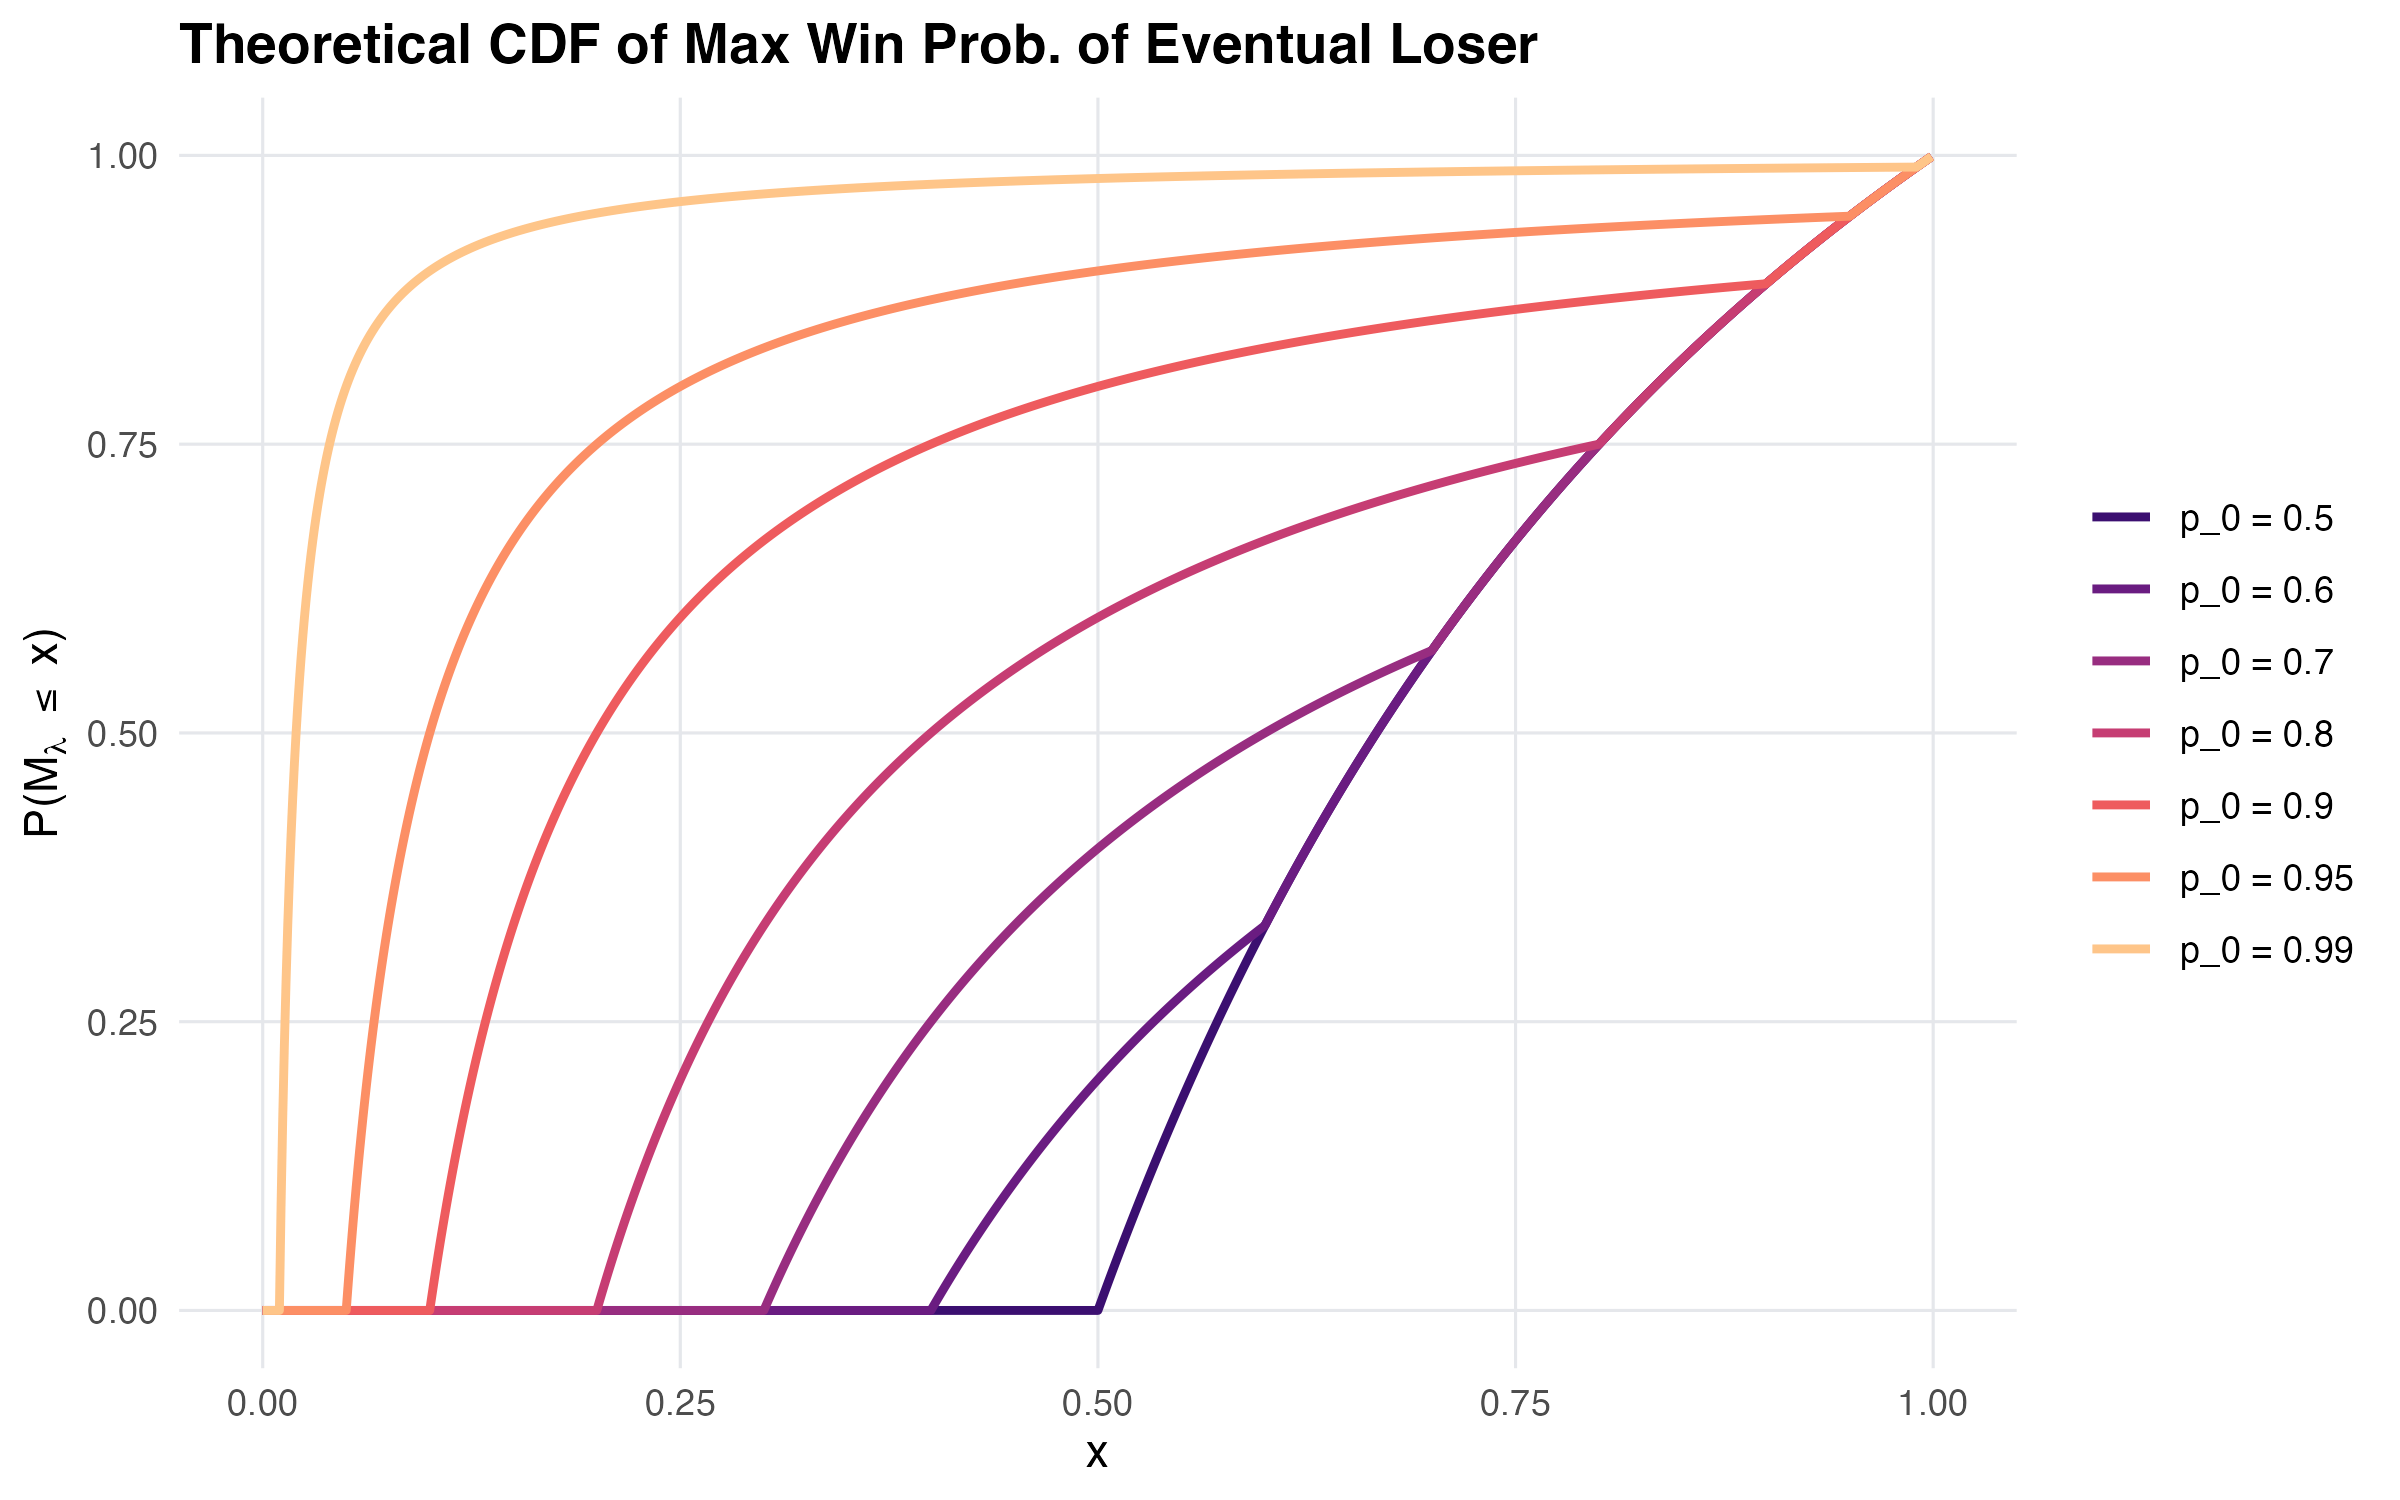
\includegraphics[width=0.8\textwidth]{figures/distributions/sports_cdf.png}
\caption{Benchmark CDF $F_{M_\lambda}(x)$ for different pre-game favorite probabilities $p_0$.}
\label{fig:sports-cdf}
\end{figure}

\subsection{Winner's trough in $n$-team contests} \label{sec:n-player}

Now consider $n\ge 3$ teams with exactly one winner.
Let $Y^{(i)}=\mathbf 1\{\text{team } i \text{ wins}\}$ and let
\[
p^{(i)}_t=\P(Y^{(i)}=1\mid\mathcal F_t),\qquad i=1,\ldots,n,
\]
be the corresponding win-probability martingales, with $\sum_{i=1}^n p^{(i)}_t=1$.
If $W$ denotes the eventual winner, the \emph{winner's trough} is simply the minimum probability assigned to the winner along the path:
\[
M_\omega:=\inf_{t\in[0,1]} p^{(W)}_t
\;=\;
\inf_{t\in[0,1]}\sum_{i=1}^n p^{(i)}_t\,\mathbf 1\{Y^{(i)}=1\}.
\]
Its benchmark distribution follows by applying Theorem~\ref{thm:continuous-conditional} to the complement martingale $1-p^{(i)}_t=\P(Y^{(i)}=0\mid\mathcal F_t)$ on the event $\{Y^{(i)}=1\}$ and then mixing over $i$ (derivation in Appendix~\ref{app:n-player-derivation}).

In the symmetric case $p^{(i)}_0=1/n$, we obtain the closed form
\[
F_{M_\omega}(x)=\frac{(n-1)x}{1-x},\qquad x\in\Big[0,\frac{1}{n}\Big),
\]
with $F_{M_\omega}(x)=1$ for $x\ge 1/n$.
For example, when $n=3$, $\P(M_\omega\le 0.2)=0.5$.
Figure~\ref{fig:nplayer-cdf} plots $F_{M_\omega}$ for several $n$.

More generally, when the pre-game probabilities $\{p^{(i)}_0\}$ are not equal, a convenient expression is
\[
F_{M_\omega}(x)
=\sum_{i=1}^n p^{(i)}_0\;\min\!\left\{1,\ \left(\frac{1-p^{(i)}_0}{p^{(i)}_0}\right)\left(\frac{x}{1-x}\right)\right\},
\qquad x\in[0,1),
\]
which reduces to the symmetric formula above when $p^{(i)}_0\equiv 1/n$.

\begin{figure}[!htbp]
\centering
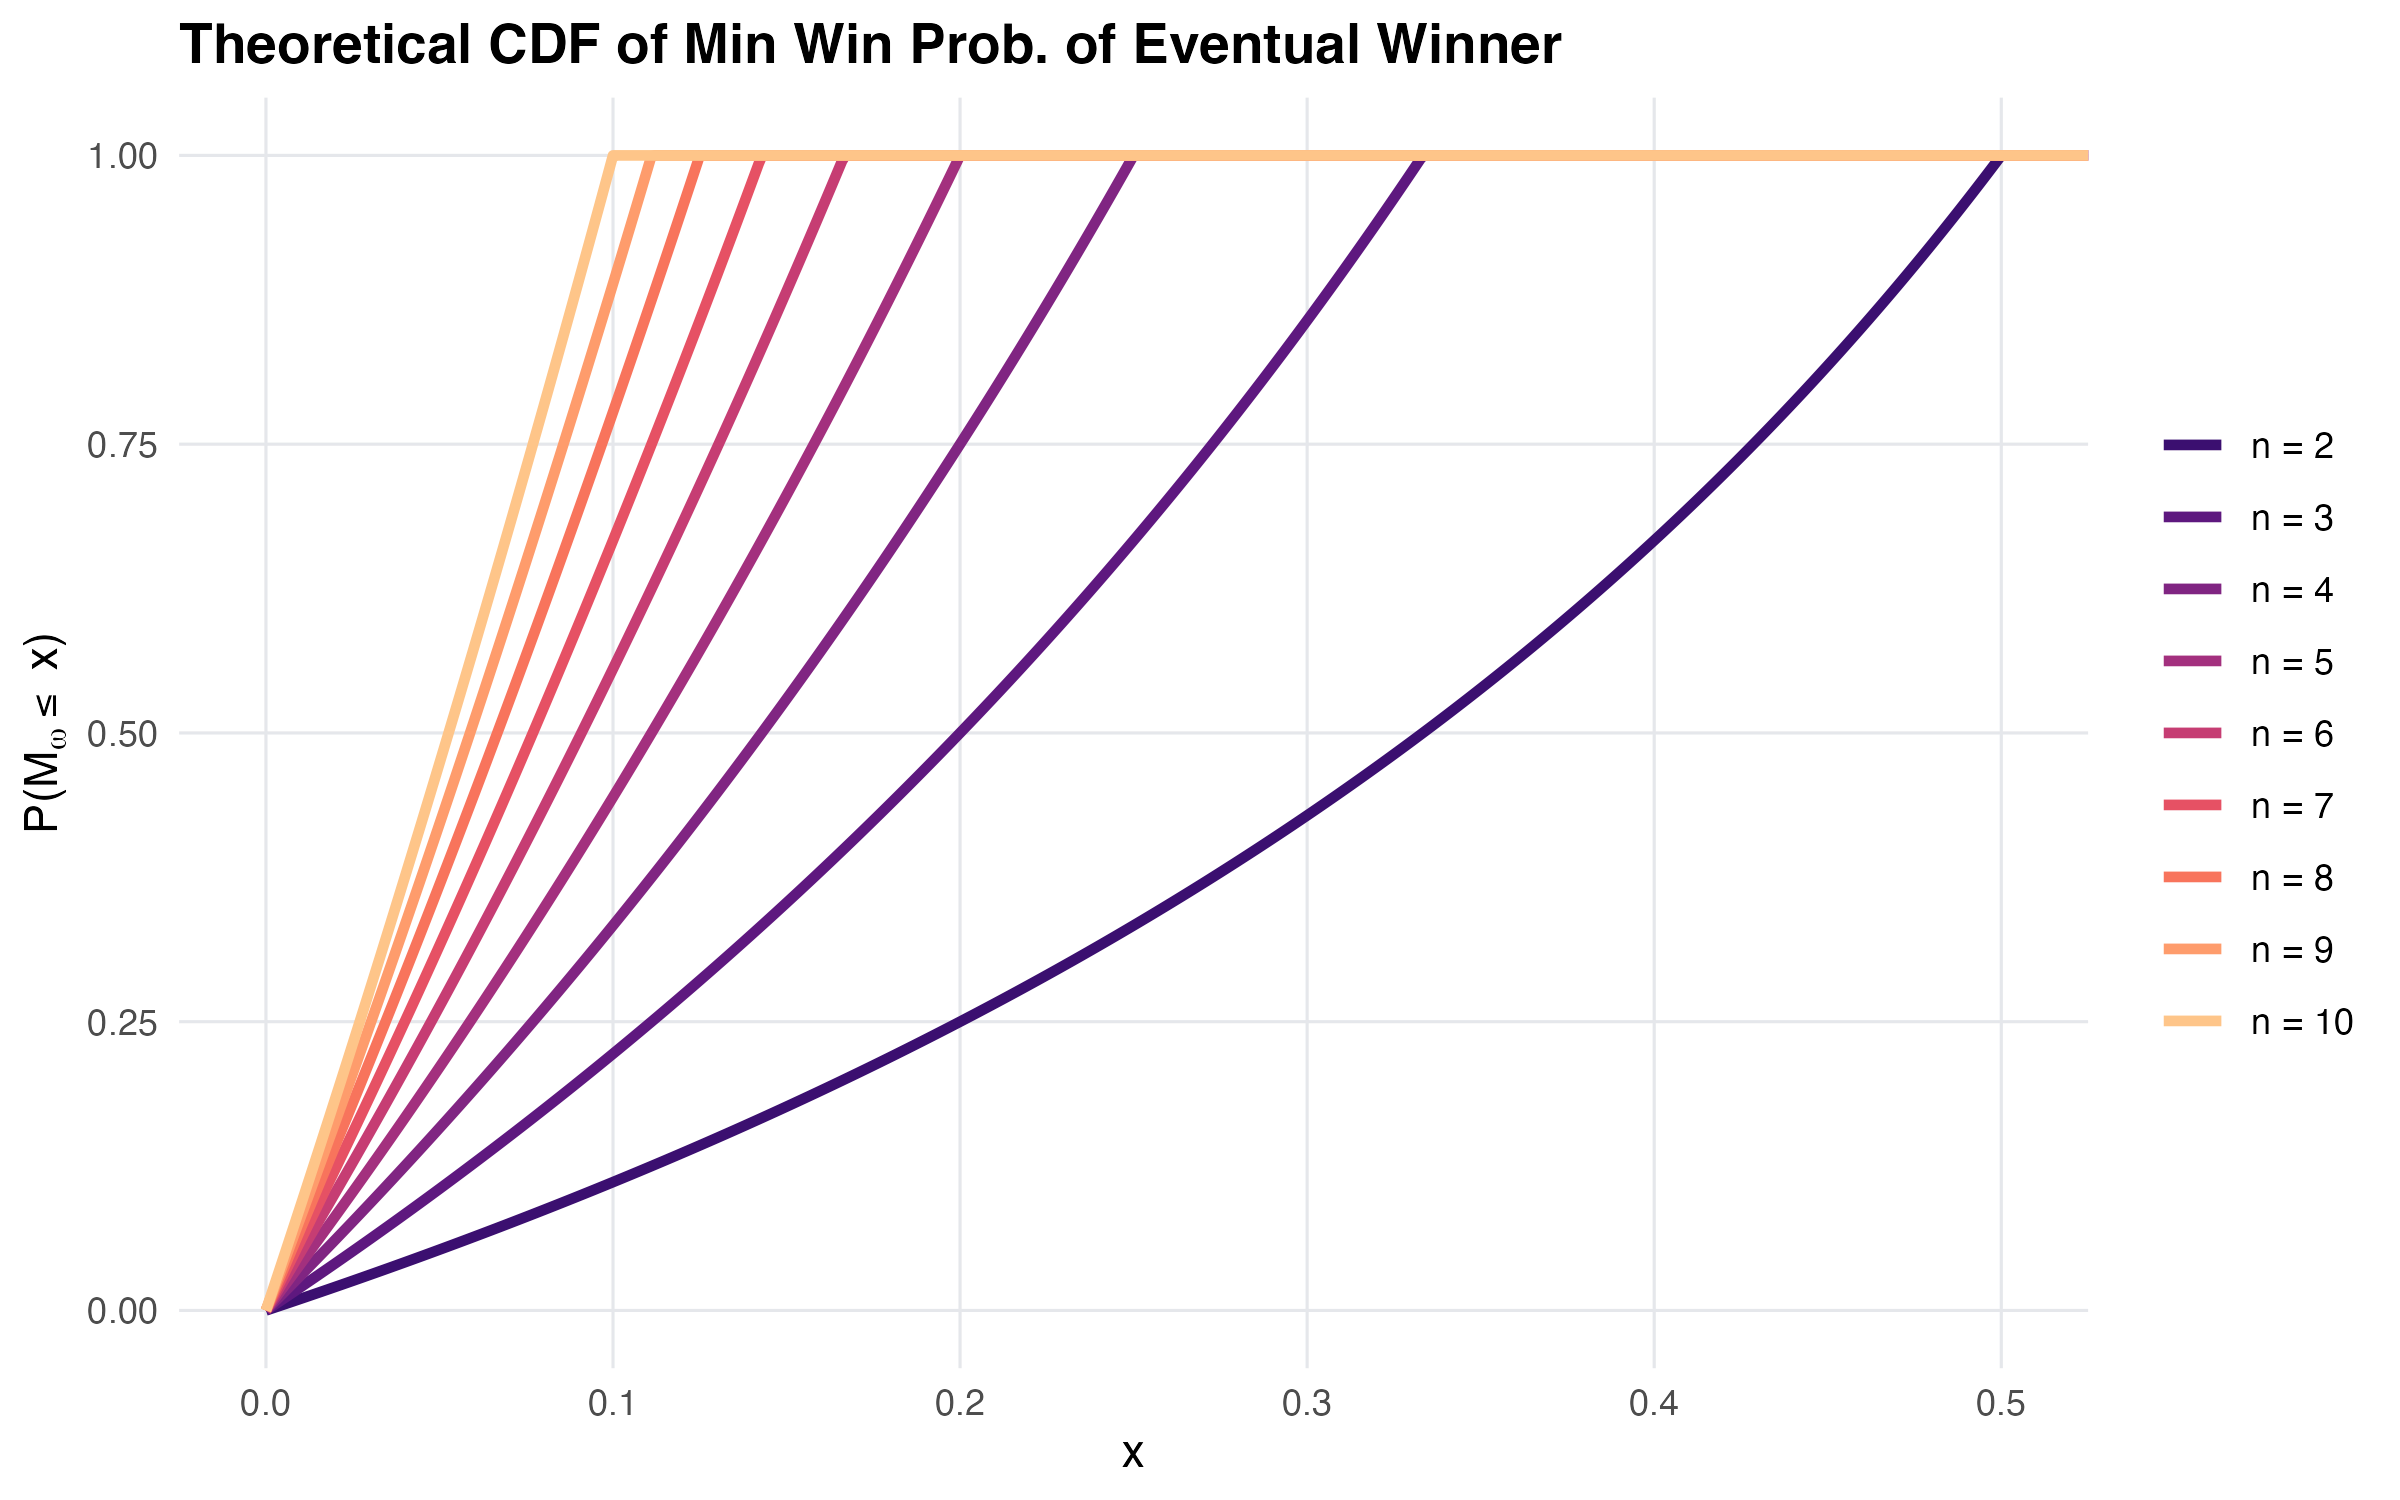
\includegraphics[width=0.8\textwidth]{figures/distributions/nplayer_cdf.png}
\caption{Benchmark CDF $F_{M_\omega}(x)$ for symmetric $n$-team games.}
\label{fig:nplayer-cdf}
\end{figure}

\subsection{Interpretation}

These corollaries calibrate common retrospective statements in competitive forecasting.
For example, ``the eventual loser was assigned $90\%$'' can have substantial null probability; similarly, the winner's trough quantifies how low the eventual winner's probability can plausibly fall.
Additional benchmark values for common thresholds are collected in Appendix~\ref{app:numerical}.
Section~\ref{sec:empirical} aggregates these game-level quantities through PIT diagnostics.

\section{Simulation study} \label{sec:simulation}

This section has three goals: (i) verify null calibration under $K$ refinement, (ii) quantify discrete-time conservatism under feed coarsening, and (iii) map structural alternatives to directional PIT signatures.

\subsection{Design}

For each trajectory $i$, we draw $p_{0,i}\sim\mathrm{Unif}(0.25,0.75)$ and $Y_i\sim\mathrm{Bernoulli}(p_{0,i})$.
Let $B_i^0(t)$ be a standard Brownian bridge on $[0,1]$, independent of $Y_i$, and define the latent signal
\[
X_i(t)=tY_i+\sigma B_i^0(t),\qquad t\in[0,1],\quad \sigma=0.5.
\]
Because $B_i^0(1)=0$, we have $X_i(1)=Y_i$.
For $t<1$, the posterior log-odds process is
\[
\ell_i(t)=\operatorname{logit}(p_{0,i})+\frac{X_i(t)-t/2}{\sigma^2(1-t)},
\qquad
p_i(t)=\operatorname{logit}^{-1}\!\big(\ell_i(t)\big),
\]
and we set $p_i(1):=Y_i$.
This gives an anchored latent null with continuous paths on $[0,1)$ and terminal revelation at $t=1$.
For the main discrete-feed experiments (coarsening and structural alternatives), we use
\[
t_k^{\mathrm{base}}=\frac{k}{K_{\mathrm{base}}},\quad k=0,\dots,K_{\mathrm{base}},\quad K_{\mathrm{base}}=1000.
\]
For null calibration, we separately refine $K$ over $\{100,1000,10000,100000,1000000\}$ at fixed $n=10000$.

To study departures from the ideal process, we map each latent path $p_i(t_k)$ to a reported path $\hat p_i(t_k)$ on a generic grid $k=0,\dots,K$ using the following operators:
\begin{itemize}[leftmargin=*, itemsep=2pt, topsep=4pt]
\item \textbf{Over/underreaction:} $\hat \ell_i(t_k)=\beta \ell_i(t_k)$.
\item \textbf{Predictable drift:} $\hat \ell_i(t_k)=\ell_i(t_k)+\delta\, t_k\tanh(\ell_i(t_k)/c)$ with $c=2$.
\item \textbf{Filtration lag:} $\hat p_i(t_k)=p_i(r_\eta(t_k))$, where $r_\eta(t)=t/(1+\eta(1-t))$ and $\eta$ indexes lag intensity: $\eta=0$ is no lag (null), and larger $\eta$ implies greater lag.
\item \textbf{Smoothing:} $\hat p_{i0}=p_{0,i}$, $\hat p_{ik}=\lambda \hat p_{i,k-1}+(1-\lambda)p_i(t_k)$ for $k=1,\dots,K-1$, and $\hat p_{iK}=Y_i$.
\item \textbf{Feed coarsening and rounding:} keep every $m$th update and optionally round to a fixed grid (e.g., $0.01$ or $0.05$).
\end{itemize}
For each simulated dataset, we compute peak-on-loss PIT values $U_i$ and summarize them with upper-tail frequencies, $D_n^{\mathrm{upper}}$, and $D_n^{\mathrm{lower}}$.

\subsection{Null calibration via $K$ refinement}

Under the true continuous-process null, PIT values are uniform by Theorem~\ref{thm:continuous-conditional}.
Figure~\ref{fig:sim-null-k} evaluates this calibration by plotting the null signature $t-\hat F_U(t)$ over an order-of-magnitude refinement range $K\in\{100,1000,10000,100000,1000000\}$ with fixed $n=10000$.
As $K$ increases, the curves move toward the reference line at zero, matching the expected convergence to the continuous-path benchmark.

\begin{figure}[!htbp]
\centering
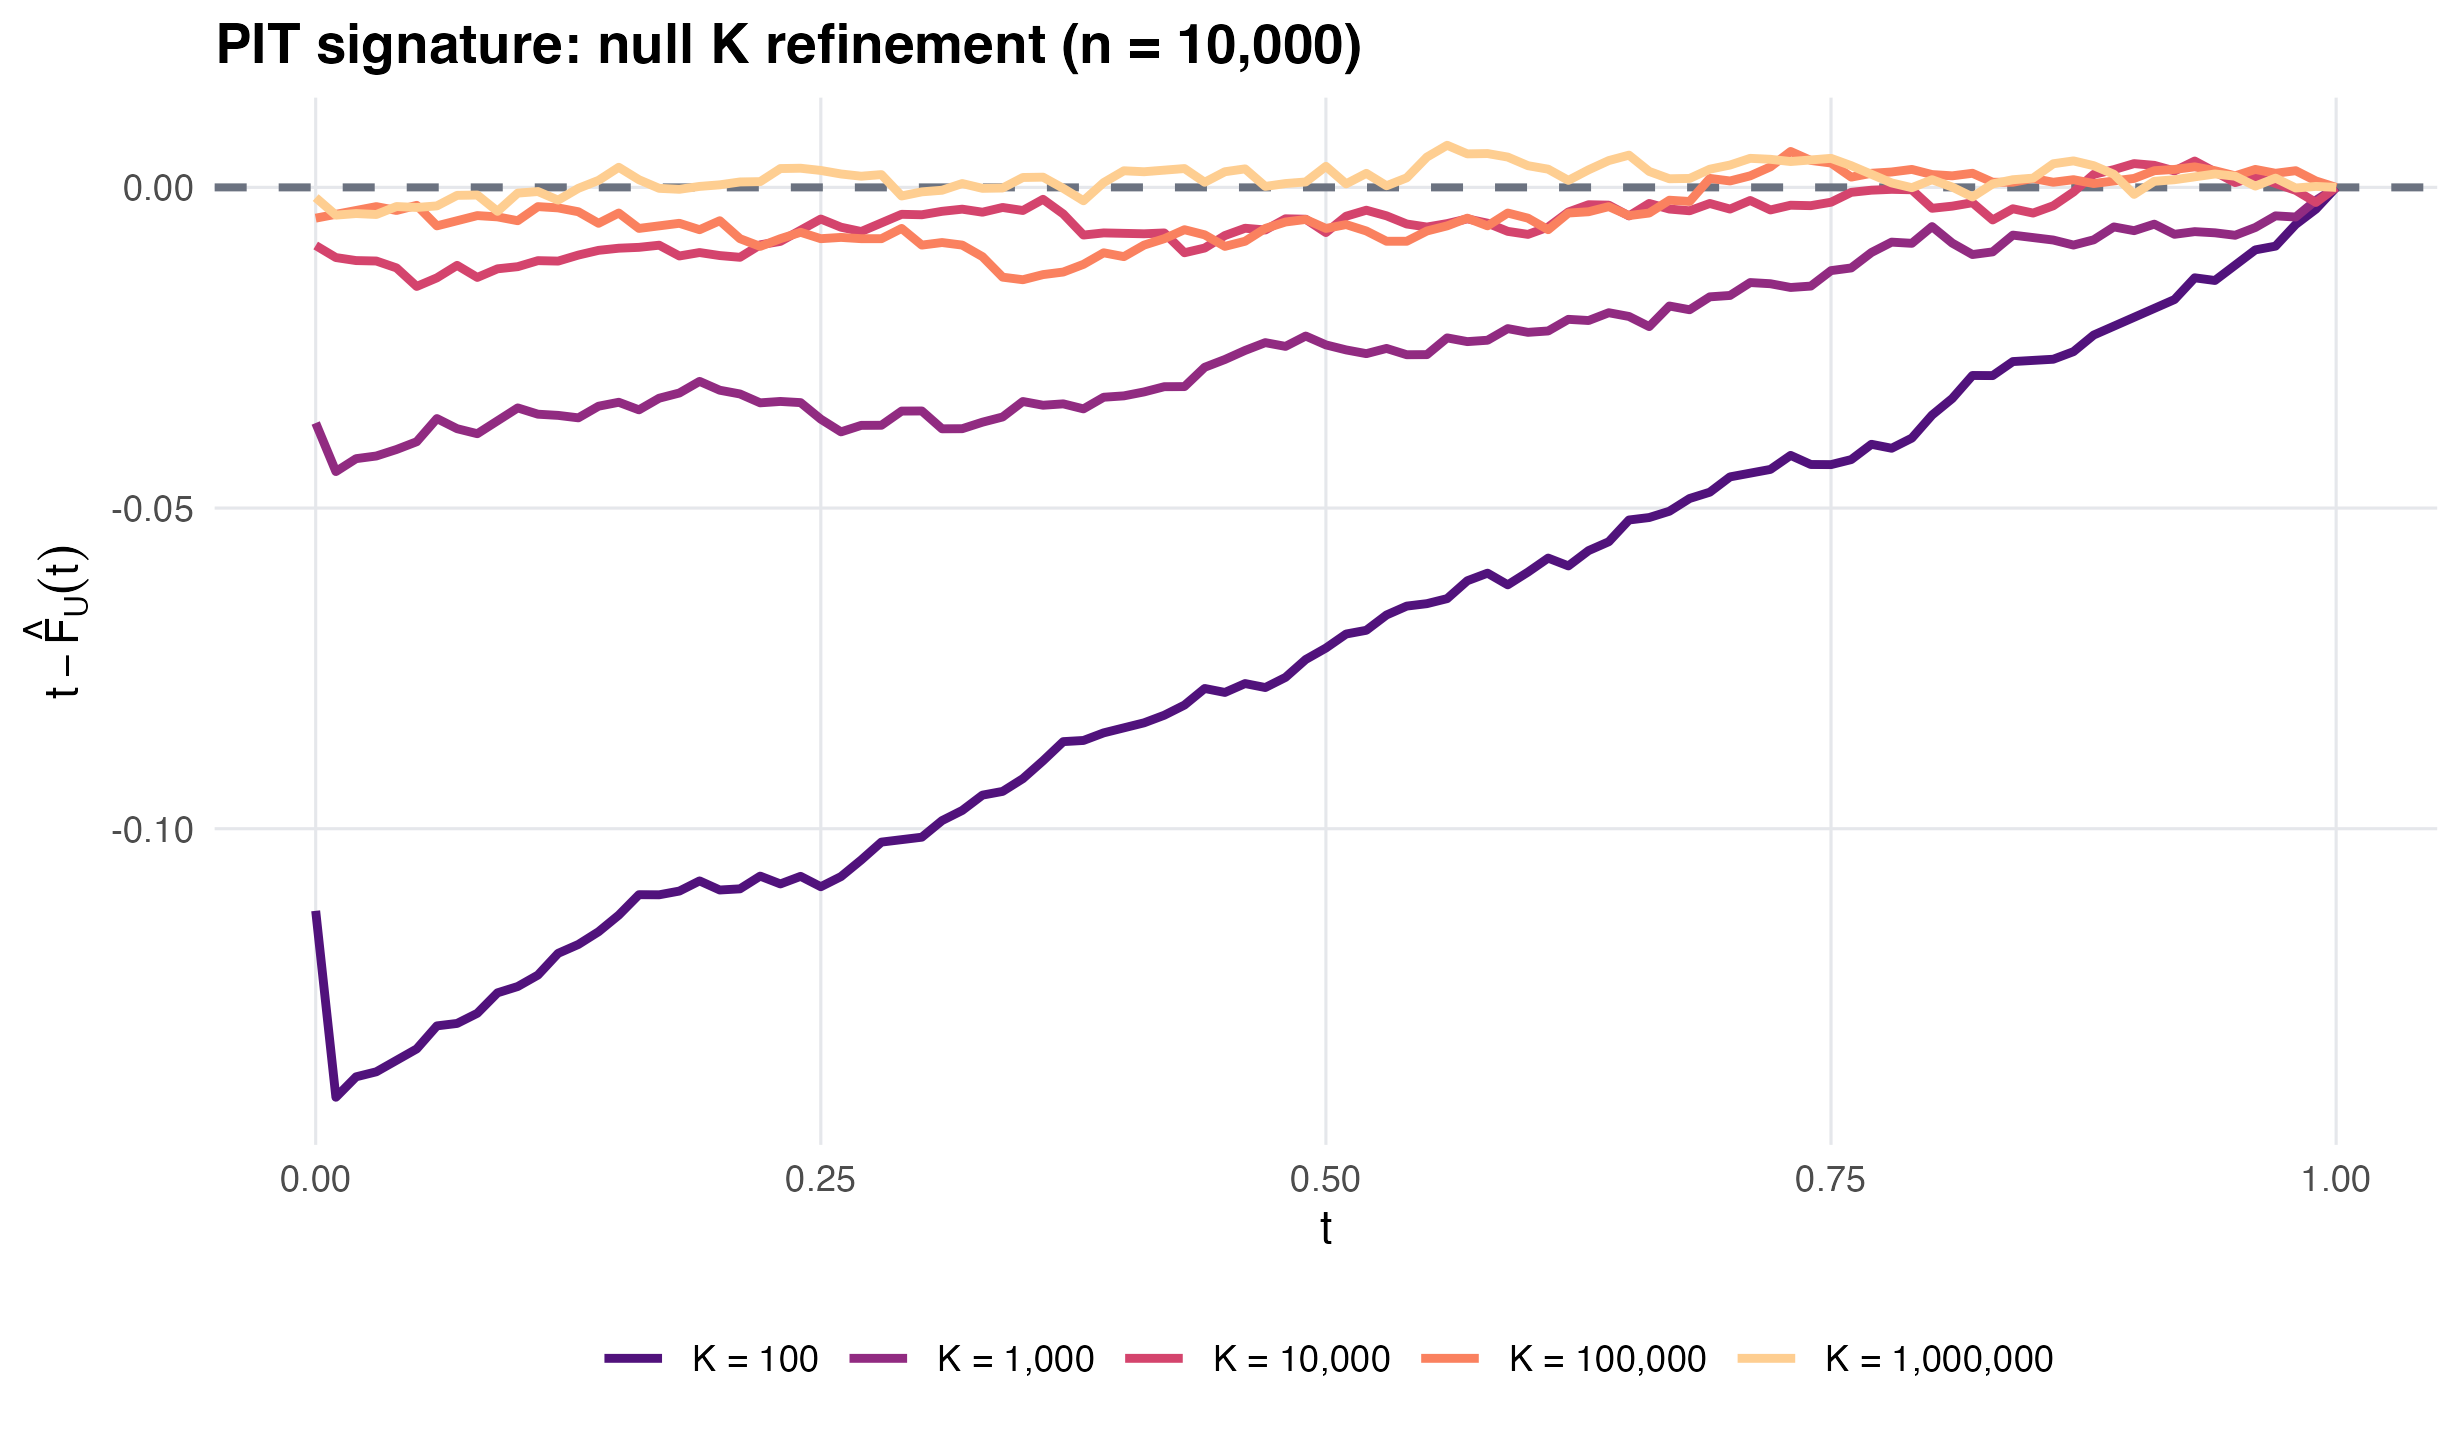
\includegraphics[width=0.82\textwidth]{figures/simulation/null_k_convergence.png}
\caption{Null calibration under $K$ refinement at fixed sample size $n=10000$: the signature $t-\hat F_U(t)$ approaches the zero reference line as the feed is refined.}
\label{fig:sim-null-k}
\end{figure}

\subsection{Discrete-time conservatism under coarsening}

Figure~\ref{fig:sim-null-gap} fixes a calibrated base process ($K_{\mathrm{base}}=1000$) and coarsens the observed feed by keeping every $m$th update.
As coarsening increases, the signature $t-\hat F_U(t)$ shifts below zero, indicating conservative upper tails under discrete observation.
The upper-tail frequencies $\widehat{\P}(U\ge u)$ decline with coarsening for $u\in\{0.90,0.95,0.99\}$, consistent with Theorem~\ref{thm:discrete-conditional}.

\begin{figure}[!htbp]
\centering
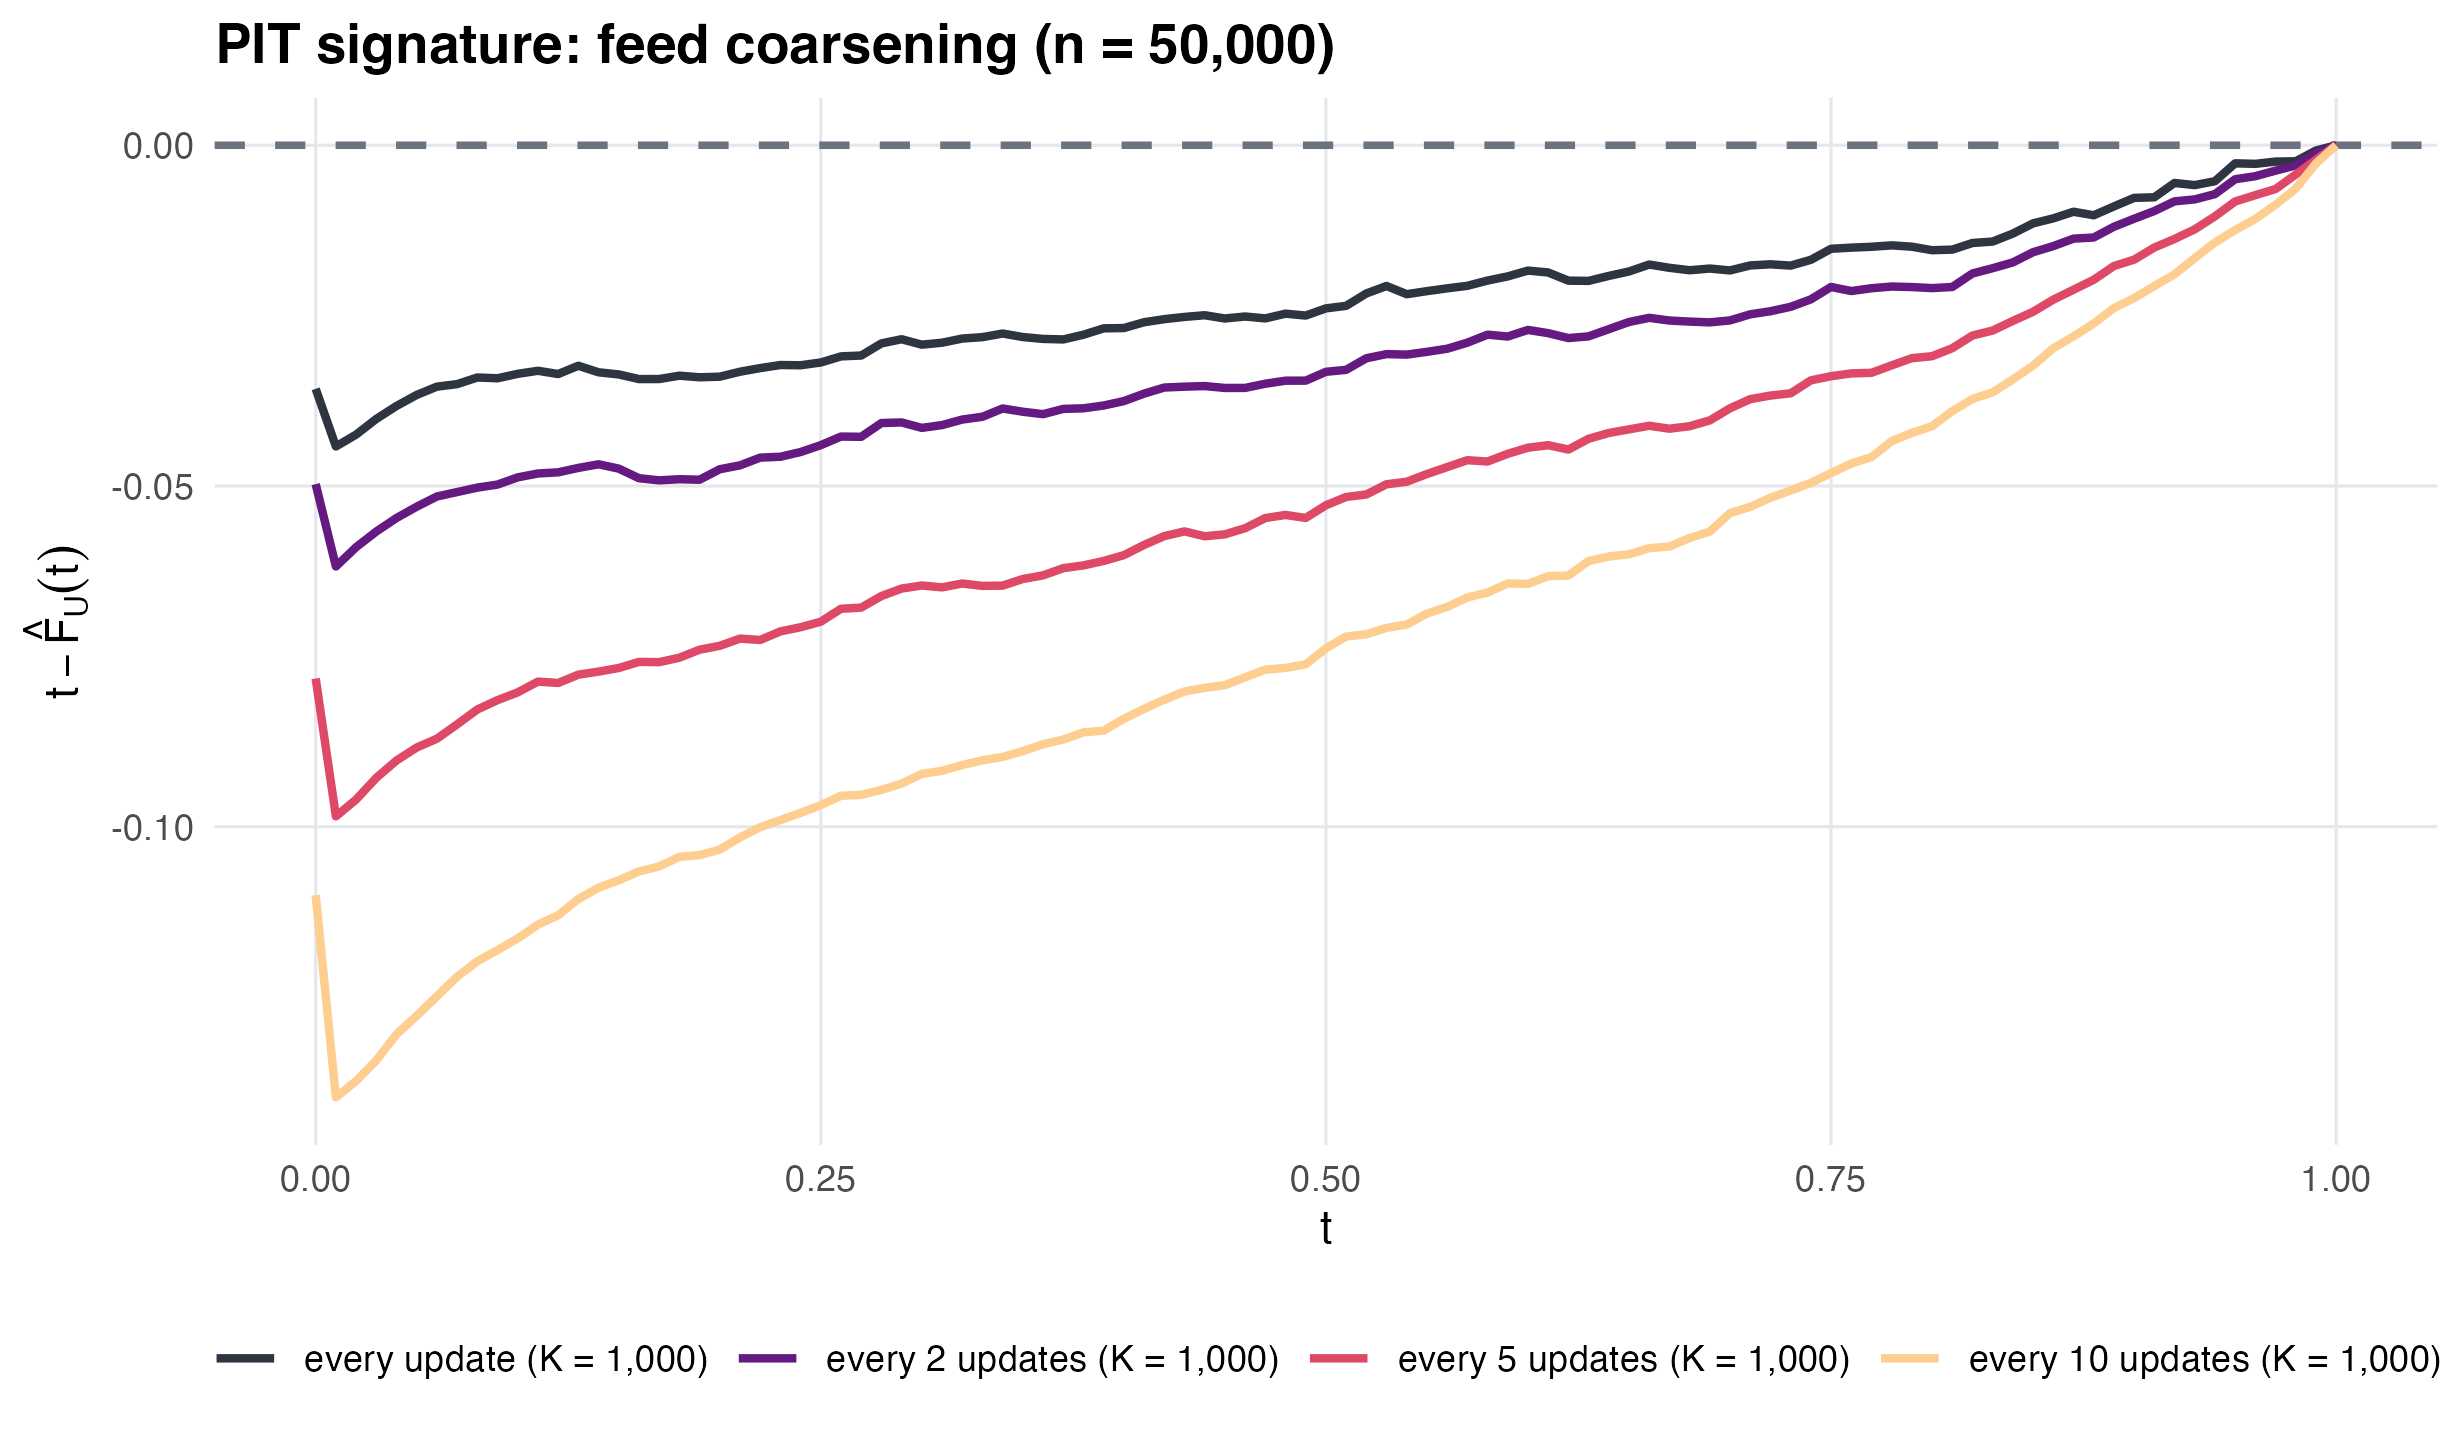
\includegraphics[width=0.82\textwidth]{figures/simulation/null_conservatism.png}
\caption{Null PIT signatures across coarsened feed resolutions from a common base process ($K_{\mathrm{base}}=1000$). Coarsening induces conservative upper tails.}
\label{fig:sim-null-gap}
\end{figure}

\subsection{Structural alternatives and directional signatures}

Figure~\ref{fig:sim-signatures} plots $t-\hat F_U(t)$ under representative alternatives.
Overreaction and positive drift produce upward deviations (excess large $U_i$), while underreaction, smoothing, and filtration lag produce the opposite directional pattern.
Curves can start slightly below zero near $t=0$ because discrete/coarsened observation induces mild null conservatism in the lower tail (so $\hat F_U(t)>t$ for very small $t$).
Coarsening mainly shifts the curve toward conservatism without mimicking the overreaction signature.

Table~\ref{tab:sim-rejections} reports estimated rejection rates at level $0.05$ for both $D_n^{\mathrm{upper}}$ and $D_n^{\mathrm{lower}}$.
To account for discrete-time conservatism, the critical values are calibrated from repeated null draws at each sample size.
The table uses path sample sizes $n\in\{1000,5000\}$, with 120 Monte Carlo replicates at $n=1000$ and 100 replicates at $n=5000$.
Because conservative validity is directional in the upper-tail statistic, we treat $D_n^{\mathrm{upper}}$ as the primary inferential target; $D_n^{\mathrm{lower}}$ is reported as a directional sensitivity diagnostic.
The resulting profile remains interpretable: $D_n^{\mathrm{upper}}$ is most sensitive to overreaction/drift (e.g., $\beta=1.1$: $0.475$ at $n=1000$, $1.000$ at $n=5000$), while $D_n^{\mathrm{lower}}$ is strongest for smoothing and underreaction (e.g., $\lambda=0.8$: $1.000$ at both sizes; $\beta=0.9$: $0.400$ at $n=1000$, $0.680$ at $n=5000$), and can also rise for strong overreaction at larger $n$.
A broader stress-test grid with additional parameter levels and reporting-artifact variants appears in Appendix Table~\ref{tab:sim-rejections-full}.

\begin{figure}[!htbp]
\centering
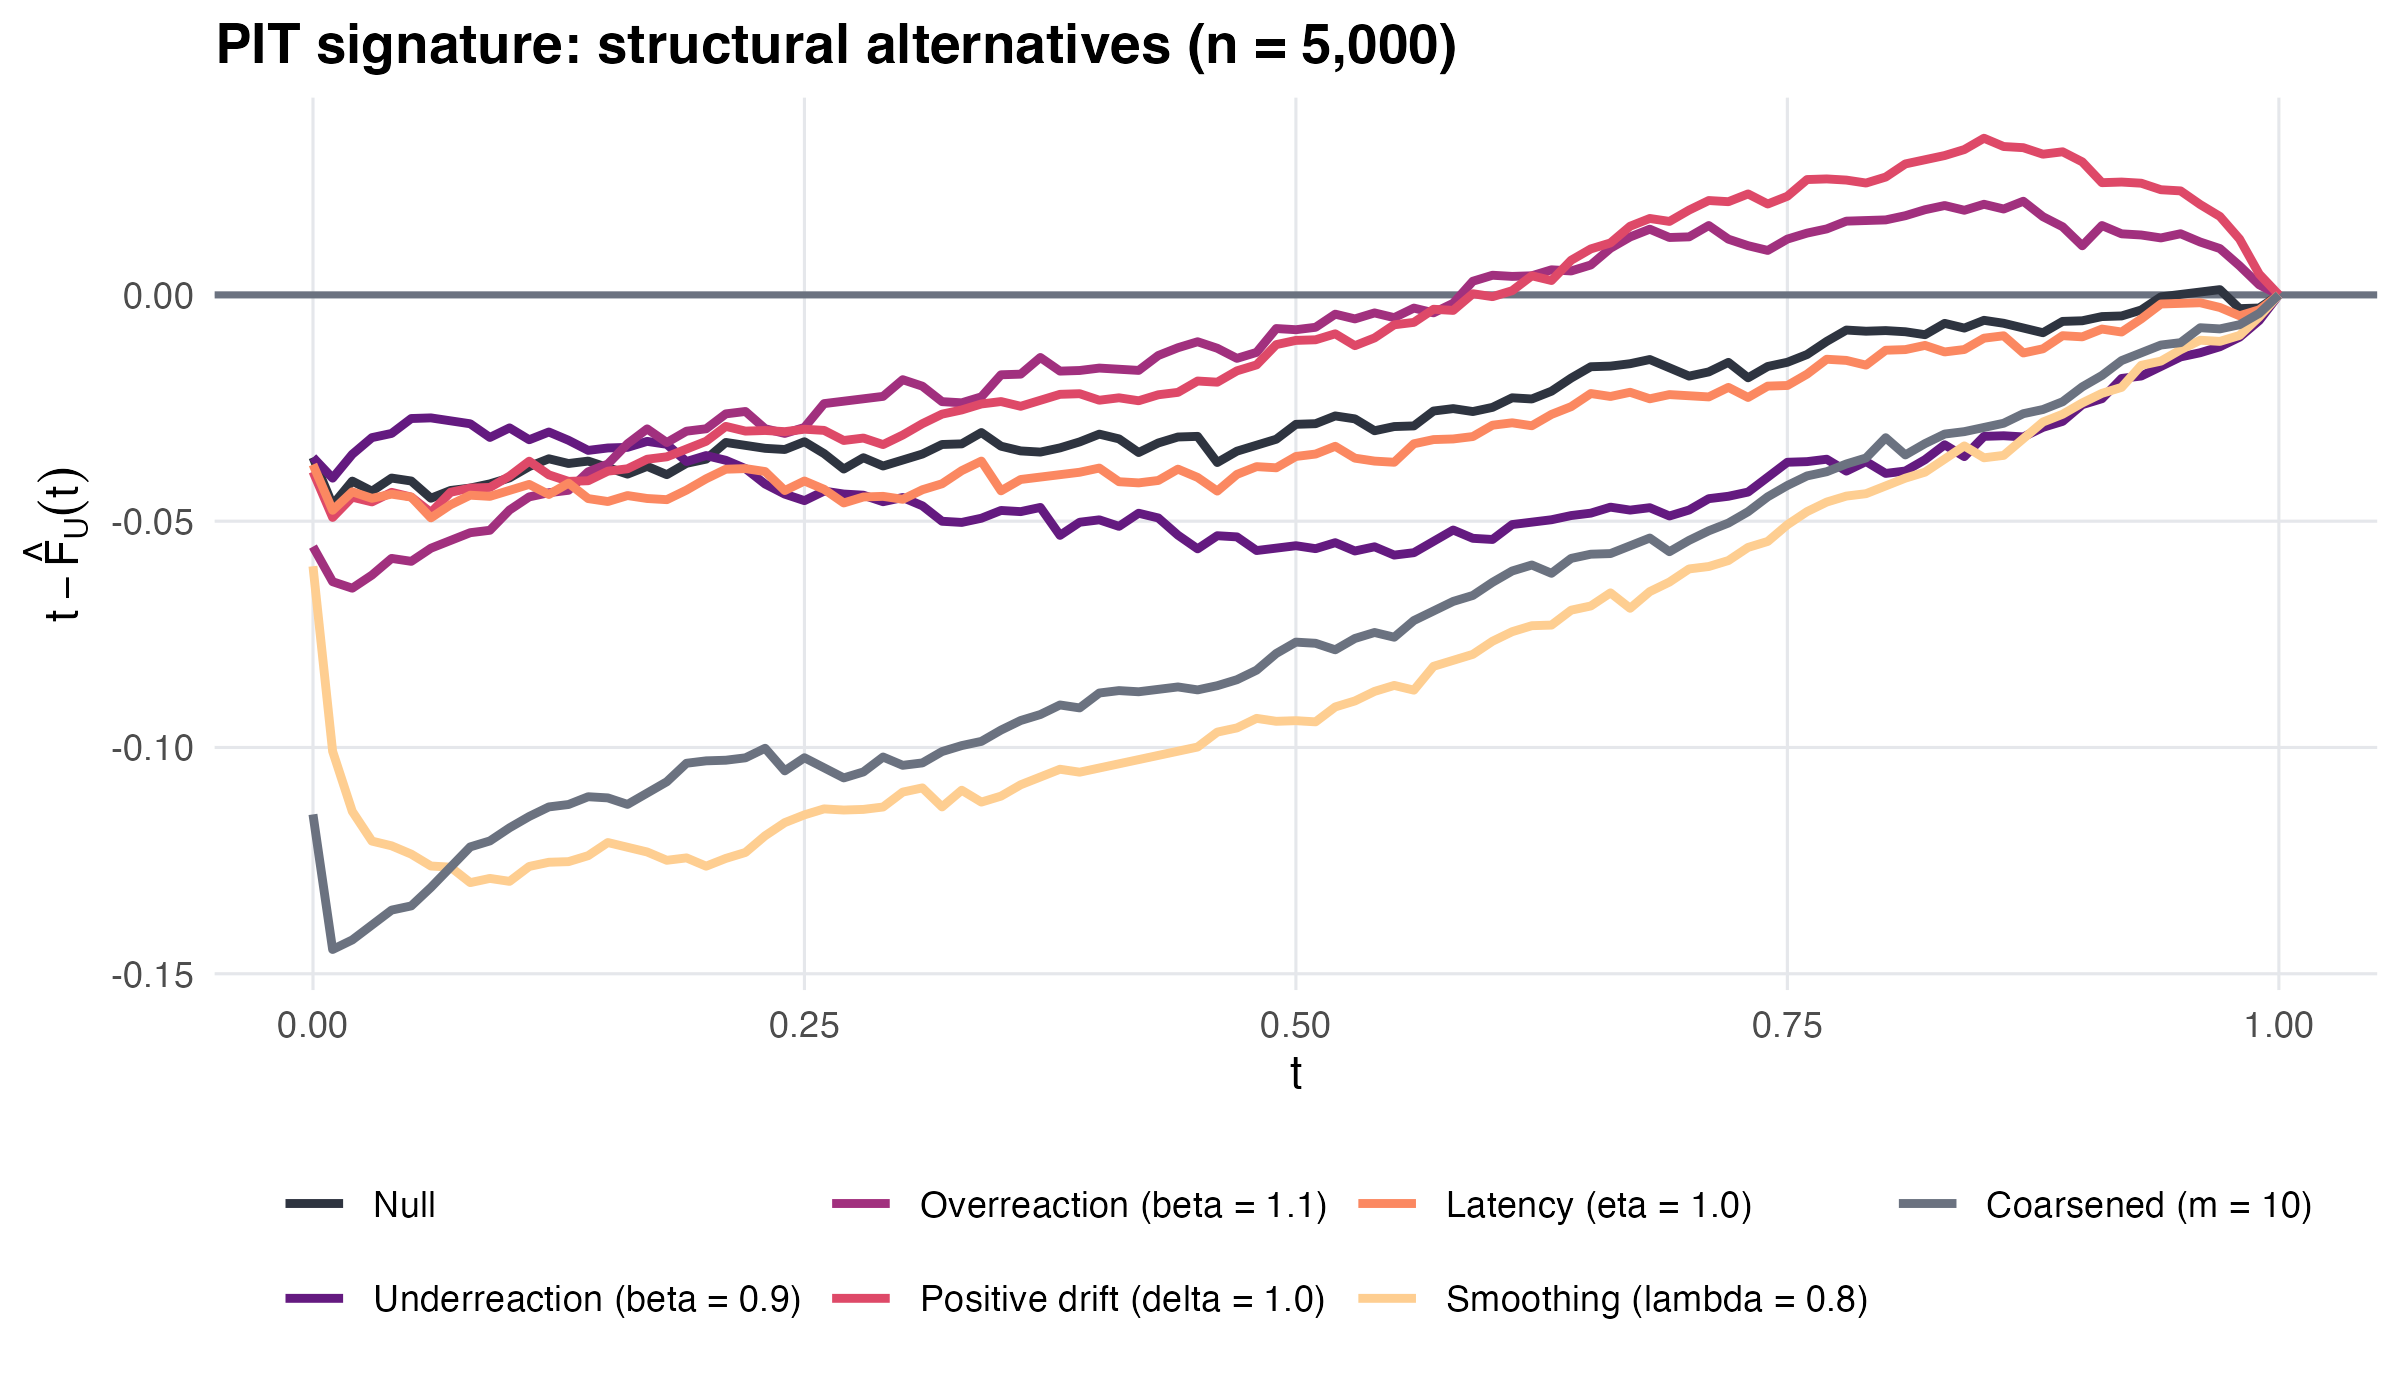
\includegraphics[width=0.82\textwidth]{figures/simulation/alternative_signatures.png}
\caption{Directional PIT signatures under representative deviations from the martingale ideal.}
\label{fig:sim-signatures}
\end{figure}

\begin{table}[!htbp]
\centering
\small
\setlength{\tabcolsep}{4pt}
\caption{Rejection rates for $D_n^{\mathrm{upper}}$ and $D_n^{\mathrm{lower}}$ under structural alternatives ($\alpha=0.05$).}
\label{tab:sim-rejections}
\begin{tabular}{lcccc}
\hline
Scenario & $D_n^{\mathrm{upper}}$ ($n=1000$) & $D_n^{\mathrm{upper}}$ ($n=5000$) & $D_n^{\mathrm{lower}}$ ($n=1000$) & $D_n^{\mathrm{lower}}$ ($n=5000$) \\
\hline
Null & 0.050 & 0.050 & 0.050 & 0.050 \\
$\beta=0.9$ & 0.000 & 0.000 & 0.400 & 0.680 \\
$\beta=1.1$ & 0.475 & 1.000 & 0.142 & 0.970 \\
$\delta=0.5$ & 0.300 & 0.950 & 0.058 & 0.070 \\
$\delta=1.0$ & 0.750 & 1.000 & 0.042 & 0.090 \\
$\eta=1.0$ & 0.033 & 0.020 & 0.150 & 0.240 \\
$\lambda=0.5$ & 0.000 & 0.000 & 0.733 & 1.000 \\
$\lambda=0.8$ & 0.000 & 0.000 & 1.000 & 1.000 \\
\hline
\end{tabular}
\end{table}

\section{Empirical study: ESPN win-probability models in the NFL and NBA} \label{sec:empirical}

This section illustrates the diagnostics on a widely visible forecasting system: live ESPN win probabilities.
The aim is methodological: test whether observed path extremes match the null predictions.

\subsection{Data sources and preprocessing}

We analyze ESPN play-by-play win-probability data for NFL and NBA regular-season games from 2018--2024 \citep{ESPN2025}.
NFL data were obtained via \texttt{espnscrapeR} \citep{espnscrapeR2025}, and NBA data via \texttt{hoopR} \citep{hoopR2023}.
After excluding ties and games with missing scores or win-probability series, we retain $n=1832$ NFL games and $n=8261$ NBA games.
For each game, we define $p_0$ as the maximum of the two teams' first-reported win probabilities (so that $p_0 \ge 0.5$) and compute $M_\lambda$ as the maximum win probability attained by the eventual loser over the game (Section~\ref{sec:loser-max-wp}).

\subsection{Null comparison via probability integral transform}

Because the benchmark distribution of $M_\lambda$ depends on $p_0$, we aggregate across games using a probability integral transform.
For game $i$, let $p_{0,i}\ge 1/2$ be the initial reported favorite probability and let $m_i=M_{\lambda,i}$ be the observed eventual-loser peak.
Define
\[
U_i := F_{M_\lambda}(m_i; p_{0,i}).
\]
Under the continuous-path law, $\{U_i\}$ are i.i.d.\ $\mathrm{Unif}(0,1)$.
For discretely updated feeds, the upper tail of $\{U_i\}$ is conservative (as predicted by Theorem~\ref{thm:discrete-conditional} and confirmed in Section~\ref{sec:simulation}), so excess large values indicate overly extreme eventual-loser peaks.
We summarize $\{U_i\}$ through the centered signature $t-\hat F_U(t)$ and note the equivalent reparameterization $P_i=1-U_i$.

\subsection{Global test and tail summaries}

Our primary global diagnostic is upper-tail inflation.
Let $\hat F_U$ be the empirical CDF of $\{U_i\}_{i=1}^n$ and define
\[
D_n^{\mathrm{upper}} := \sup_{0\le t\le 1}\{t-\hat F_U(t)\}.
\]
Large $D_n^{\mathrm{upper}}$ indicates excess large $U_i$ values; this direction remains valid under discrete-time conservatism.

As descriptive complements, we report
$\widehat{\P}_n(U\ge u)$ for $u\in\{0.90,0.95,0.99\}$; values substantially above
$\{0.10,0.05,0.01\}$ indicate upper-tail inflation.

Figure~\ref{fig:pit-combined} plots the centered PIT signature $t-\hat F_U(t)$ for both leagues, with a zero-reference line.
Tables~\ref{tab:ks-kl-nfl} and~\ref{tab:ks-kl-nba} report $D_n^{\mathrm{upper}}$, its one-sided $p$-value, and the tail summaries.

\begin{figure}[!htbp]
\centering
\begin{subfigure}[t]{0.8\textwidth}
  \centering
  
\includegraphics[width=\textwidth]{figures/nfl/pit.png}
  \subcaption{NFL}
  \label{fig:nfl-pit}
\end{subfigure}\\[0.5em]
\begin{subfigure}[t]{0.8\textwidth}
  \centering
  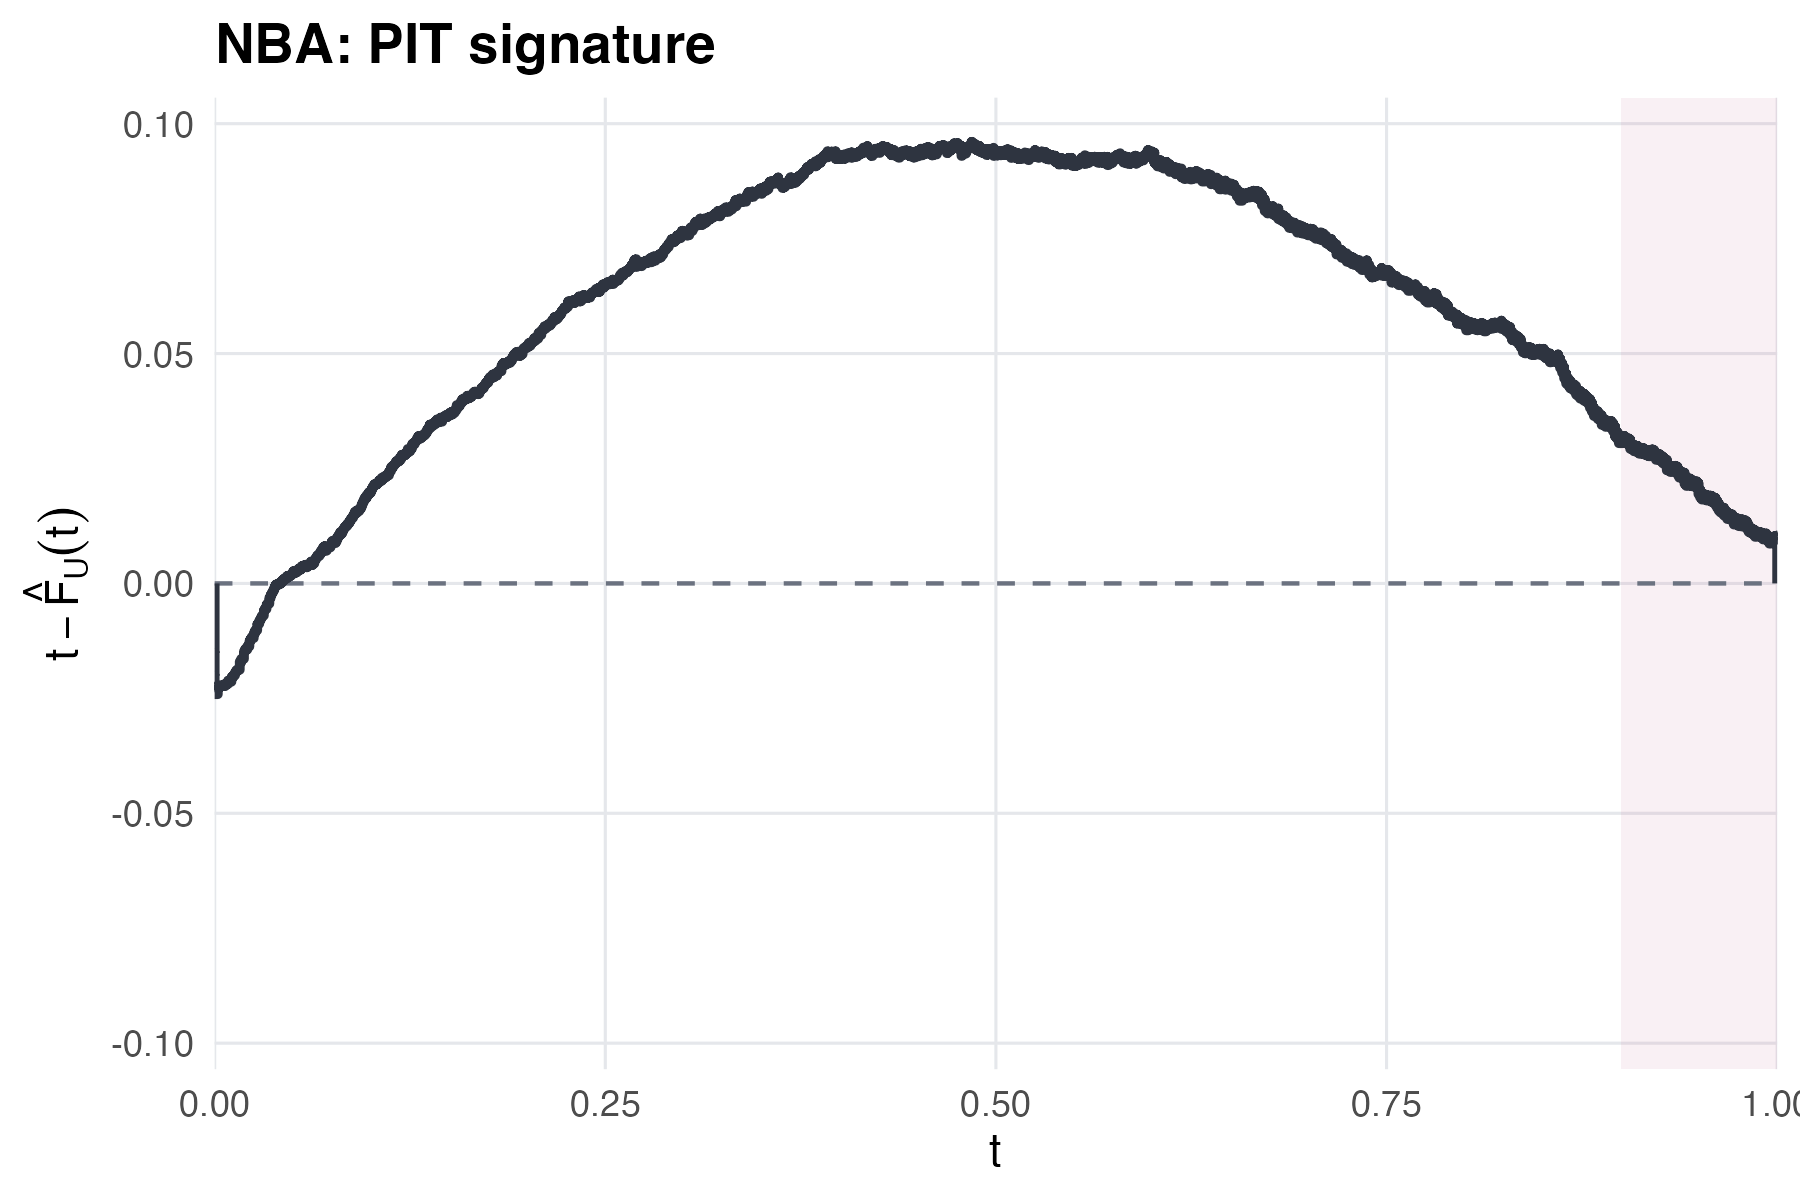
\includegraphics[width=\textwidth]{figures/nba/pit.png}
  \subcaption{NBA}
  \label{fig:nba-pit}
\end{subfigure}
\caption{Centered PIT signatures $t-\hat F_U(t)$ with the zero-reference line.}
\label{fig:pit-combined}
\end{figure}

\begin{table}[!htbp]
\caption{NFL PIT diagnostic summary.}
\label{tab:ks-kl-nfl}
\centering
\begin{tabular}{lccccc}
\hline
$n$ & $\widehat{\P}_n(U \ge 0.90)$ & $\widehat{\P}_n(U \ge 0.95)$ & $\widehat{\P}_n(U \ge 0.99)$ & $D_n^{\mathrm{upper}}$ & $p$-value \\
\hline
1832 & 0.086 & 0.046 & 0.017 & 0.0153 & 0.424 \\
\hline
\end{tabular}
\end{table}

\begin{table}[!htbp]
\caption{NBA PIT diagnostic summary.}
\label{tab:ks-kl-nba}
\centering
\begin{tabular}{lccccc}
\hline
$n$ & $\widehat{\P}_n(U \ge 0.90)$ & $\widehat{\P}_n(U \ge 0.95)$ & $\widehat{\P}_n(U \ge 0.99)$ & $D_n^{\mathrm{upper}}$ & $p$-value \\
\hline
8261 & 0.131 & 0.070 & 0.020 & 0.0962 & $<$0.0001 \\
\hline
\end{tabular}
\end{table}

\subsection{Interpretation of the diagnostic tests}

The NFL results (Table~\ref{tab:ks-kl-nfl}) show no strong evidence against the null in the tested direction.
The empirical upper-tail frequencies at $u\in\{0.90,0.95\}$ are close to nominal exceedance rates ($0.086$ vs.\ $0.10$, $0.046$ vs.\ $0.05$), while the $u=0.99$ tail is mildly elevated ($0.017$ vs.\ $0.01$).
The one-sided upper-tail K--S statistic does not reject ($p=0.42$), indicating no systematic upper-tail inflation.

The NBA results (Table~\ref{tab:ks-kl-nba}) show clear departures.
Upper-tail mass is inflated ($0.131$ vs.\ $0.10$, $0.070$ vs.\ $0.05$, $0.020$ vs.\ $0.01$), and the one-sided K--S statistic is large ($p<10^{-4}$).
We therefore reject the null in the direction of excessively high eventual-loser peaks.
This discrepancy is consistent with overconfident or overly reactive updating, but could also reflect filtration mismatch or reporting/estimation artifacts in the published series (Section~\ref{sec:discussion}).

\section{Discussion} \label{sec:discussion}

Narratives around sequential probability forecasts often emphasize retrospective extremes: ``the team reached $90\%$ and still lost.''
The relevant baseline for these statements is the \emph{conditional} law of path extrema given the terminal outcome, rather than fixed-time heuristics such as $1-m$.
This perspective turns narratives about ``peak probabilities'' into testable distributional claims.
In settings such as sports win probabilities, departures may reflect update misspecification, filtration mismatch, or publication artifacts rather than the intrinsic surprisingness of any single collapse.

\subsection{Limitations and assumptions}

Our theoretical guarantees are statements about the ideal process $p_k=\E[Y\mid\mathcal F_k]$.
In practice, reported win probabilities estimate this conditional expectation, so empirical discrepancies may also reflect model misspecification, nonstationarity, or information-set mismatch (the model's effective information set not aligning with the outcome-relevant filtration).

Exact identities additionally require continuous sample paths, which rule out terminal-time first attainment and first-passage overshoots.
For discretely updated feeds, our discrete-time results remain valid but can be conservative; the gap is governed by explicit correction terms associated with overshoots and terminal-time first attainment.
Finally, we treat binary terminal outcomes $p_N\in\{0,1\}$; extensions to ties or other non-binary terminal structures require different arguments.

\subsection{Extensions}

Several extensions are natural.
First, relax the terminal binary condition to allow $p_N\in[0,1]$ (e.g.\ ties or partial-credit outcomes).
Second, derive analogous laws for other path functionals, such as peak timing, joint laws like $(\sup_t p_t, p_1)$, or multistream extremes.
Third, extend the structured-deviation analysis beyond the one-parameter families studied here (sensitivity scaling, predictable drift, filtration lag, and smoothing) to include richer jump components and multistream interactions.
Together, these directions preserve the core perspective: conditional extreme-value laws provide a simple, model-agnostic way to evaluate sequential probability forecasts using the same peak-probability framing used in practice while retaining a principled calibration interpretation.

\newpage

\appendix
\begin{center}
\Large\bfseries Appendix
\end{center}

\section{Proofs of Discrete-Time Results} \label{app:discrete-proofs}

Throughout, $(p_k)_{k=0}^N$ is a bounded martingale with $p_0\in(0,1)$ and terminal value $p_N=Y\in\{0,1\}$.
For $x\in(0,1]$, define the first-passage time
\[
\tau_x := \inf\{k\in\{0,1,\dots,N\}: p_k\ge x\},
\]
with $\inf\varnothing := N+1$.

\subsection{Unconditional distribution of $M_N$}

\begin{theorem}[Discrete-time unconditional bound] \label{thm:supp-discrete-unconditional}
Let $M_N=\max_{0\le k\le N} p_k$. For $x\in[p_0,1)$,
\[
F_{M_N}(x)=\P(M_N\le x)\;\ge\;1-\frac{p_0}{x},
\]
with equality if $p_{\tau_x}=x$ a.s.\ on $\{\tau_x\le N\}$.
For $x<p_0$, $F_{M_N}(x)=0$.
Moreover, $M_N$ has an atom at $1$ with $\P(M_N=1)=p_0$.
\end{theorem}

\begin{proof}
If $x<p_0$ then $M_N\ge p_0>x$ a.s., hence $F_{M_N}(x)=0$.

Fix $x\in[p_0,1)$. By optional stopping for the bounded martingale $(p_k)$ at $\tau_x\wedge N$,
\[
\E[p_{\tau_x\wedge N}] = p_0.
\]
Decompose $p_{\tau_x\wedge N}=p_{\tau_x}\mathbf 1\{\tau_x\le N\}+p_N\mathbf 1\{\tau_x>N\}$.
On $\{\tau_x\le N\}$ we have $p_{\tau_x}\ge x$.
Therefore,
\[
p_0
= \E[p_{\tau_x}\mathbf 1\{\tau_x\le N\}] + \E[p_N\mathbf 1\{\tau_x>N\}]
\;\ge\; x\,\P(\tau_x\le N).
\]
Since $\{\tau_x\le N\}=\{M_N\ge x\}$, this yields
\[
\P(M_N\ge x)\le \frac{p_0}{x}\qquad\Rightarrow\qquad
F_{M_N}(x)=1-\P(M_N>x)\ge 1-\frac{p_0}{x}.
\]
Equality holds when $p_{\tau_x}=x$ a.s.\ on $\{\tau_x\le N\}$.

Finally, $M_N=1$ iff $p_N=1$ iff $Y=1$, so $\P(M_N=1)=p_0$.
\end{proof}

\subsection{Conditional distribution of $M_N$ given $Y=0$}

\begin{theorem}[Discrete-time conditional bound] \label{thm:supp-discrete-conditional}
For $x\in[p_0,1)$,
\[
F_{M_N\mid Y=0}(x)=\P(M_N\le x\mid Y=0)
\;\ge\;
1-\Big(\frac{p_0}{1-p_0}\Big)\Big(\frac{1-x}{x}\Big),
\]
with equality under the same no-overshoot condition as in Theorem~\ref{thm:supp-discrete-unconditional}.
For $x<p_0$, $F_{M_N\mid Y=0}(x)=0$.
\end{theorem}

\begin{proof}
Fix $x\in[p_0,1)$. Decompose $\P(M_N\ge x)$ by $Y$:
\[
\P(M_N\ge x)=\P(M_N\ge x, Y=1)+\P(M_N\ge x, Y=0).
\]
On $\{Y=1\}$ we have $p_N=1\ge x$, hence $\{Y=1\}\subseteq\{M_N\ge x\}$ and
\[
\P(M_N\ge x)=\P(Y=1)+\P(Y=0)\P(M_N\ge x\mid Y=0)
= p_0 + (1-p_0)\P(M_N\ge x\mid Y=0).
\]
By Theorem~\ref{thm:supp-discrete-unconditional}, $\P(M_N\ge x)\le p_0/x$, so
\[
\frac{p_0}{x}\;\ge\; p_0 + (1-p_0)\P(M_N\ge x\mid Y=0),
\]
which rearranges to
\[
\P(M_N\ge x\mid Y=0)\;\le\;\Big(\frac{p_0}{1-p_0}\Big)\Big(\frac{1-x}{x}\Big).
\]
Taking complements gives the stated lower bound on $F_{M_N\mid Y=0}(x)$.
\end{proof}

\begin{proof}[Proof of Remark~\ref{rem:discrete-correction}]
Fix $x\in(p_0,1)$. Since $x<1$, the event $\{Y=1\}$ is contained in $\{\tau_x\le N\}$, so
\[
\P(\tau_x\le N)=\P(Y=1)+(1-p_0)\P(M_N\ge x\mid Y=0).
\]
Optional stopping at $\tau_x\wedge N$ gives
\[
p_0=\E[p_{\tau_x\wedge N}]
=\E[p_{\tau_x}\mathbf 1\{\tau_x\le N\}]
=x\,\P(\tau_x\le N)+\E\!\big[(p_{\tau_x}-x)\mathbf 1\{\tau_x\le N\}\big].
\]
Combining the two displays and rearranging yields
\[
\P(M_N\ge x\mid Y=0)
=\frac{p_0}{1-p_0}\cdot\frac{1-x}{x}
-\frac{1}{x(1-p_0)}\,\E\!\big[(p_{\tau_x}-x)\mathbf 1\{\tau_x\le N\}\big].
\]
Finally,
\[
\E\!\big[(p_{\tau_x}-x)\mathbf 1\{\tau_x\le N\}\big]
=\E\!\big[(p_{\tau_x}-x)\mathbf 1\{\tau_x< N\}\big]+(1-x)\P(\tau_x=N),
\]
because $\tau_x=N$ implies $p_{\tau_x}=p_N=1$.
Substituting gives the stated decomposition.
\end{proof}

\section{Proofs of Continuous-Path Results} \label{app:continuous-proofs}

Let $(p_t)_{t\in[0,1]}$ be a bounded martingale with $p_0\in(0,1)$ and $p_1=Y\in\{0,1\}$, and assume path continuity.
Define $M=\sup_{t\in[0,1]}p_t$ and $\tau_x=\inf\{t\in[0,1]: p_t\ge x\}$.

\subsection{Unconditional distribution of $M$}

\begin{theorem}[Continuous-path unconditional] \label{thm:supp-continuous-unconditional}
For $x\in[p_0,1)$,
\[
F_M(x)=\P(M\le x)=1-\frac{p_0}{x},
\]
and $F_M(x)=0$ for $x<p_0$, while $F_M(1)=1$.
In particular, $\P(M=1)=p_0$.
\end{theorem}

\begin{proof}
If $x<p_0$ then $M\ge p_0>x$ a.s.

Fix $x\in[p_0,1)$. Optional stopping at $\tau_x\wedge 1$ yields $\E[p_{\tau_x\wedge 1}]=p_0$.
By continuity, on $\{\tau_x<1\}$ we have $p_{\tau_x}=x$, and on $\{\tau_x\ge 1\}$ we have $p_1=Y$.
Thus
\[
p_0 = x\,\P(\tau_x<1) + \E[Y\mathbf 1\{\tau_x\ge 1\}].
\]
But if $\tau_x\ge 1$ and $Y=1$, then $p_1=1\ge x$ forces $\tau_x\le 1$, a contradiction; hence
$\E[Y\mathbf 1\{\tau_x\ge 1\}]=0$ for $x<1$.
Therefore $p_0 = x\,\P(\tau_x<1)$, i.e.\ $\P(M\ge x)=\P(\tau_x<1)=p_0/x$.
The CDF follows by complement. Finally, $M=1$ iff $Y=1$, so $\P(M=1)=p_0$.
\end{proof}

\subsection{Conditional distribution of $M$ given $Y=0$}

\begin{theorem}[Continuous-path conditional] \label{thm:supp-continuous-conditional}
For $x\in[p_0,1)$,
\[
F_{M\mid Y=0}(x)=\P(M\le x\mid Y=0)
=
1-\Big(\frac{p_0}{1-p_0}\Big)\Big(\frac{1-x}{x}\Big),
\]
and $F_{M\mid Y=0}(x)=0$ for $x<p_0$, while $F_{M\mid Y=0}(1)=1$.
\end{theorem}

\begin{proof}
Fix $x\in[p_0,1)$. As before,
\[
\P(M\ge x)=\P(Y=1)+(1-p_0)\P(M\ge x\mid Y=0)=p_0+(1-p_0)\P(M\ge x\mid Y=0).
\]
By Theorem~\ref{thm:supp-continuous-unconditional}, $\P(M\ge x)=p_0/x$, hence
\[
\frac{p_0}{x}=p_0+(1-p_0)\P(M\ge x\mid Y=0)
\quad\Rightarrow\quad
\P(M\ge x\mid Y=0)=\Big(\frac{p_0}{1-p_0}\Big)\Big(\frac{1-x}{x}\Big).
\]
Taking complements yields the CDF.
Finally, on $\{Y=0\}$ the process cannot attain $1$ (if $p_t=1$ then $\P(Y=1\mid\mathcal F_t)=1$), so $M<1$ a.s.\ and $F_{M\mid Y=0}(1)=1$.
\end{proof}

\section{Distribution of \texorpdfstring{$M_\lambda$}{M\_lambda} (Two Teams)} \label{app:two-player-derivation}

Recall the two-team setting with win-probability martingales $(p_t)$ and $(q_t)$, where $q_t = 1 - p_t$ and $p_0 = \P(Y=1)$; assume $p_0 \ge 0.5$ without loss of generality.
The maximum win probability attained by the eventual loser is
\begin{equation} \label{eq:supp-M-lambda-def}
    M_\lambda \equiv \sup_{0 \leq t \leq 1} \Big( p_t \boldsymbol{1}\{Y = 0\} + q_t \boldsymbol{1}\{Y = 1\} \Big).
\end{equation}
By the law of total probability,
\begin{align} \label{eq:supp-M-lambda-total-prob}
    F_{M_\lambda}(x) = \P(M_\lambda \le x) &= \P(M_\lambda \le x \mid Y=0) (1-p_0) + \P(M_\lambda \le x \mid Y=1) p_0.
\end{align}

From the conditional distributions of the previous section, when team~A loses we have
\begin{align}
    F_{M_\lambda \mid Y=0}(x) = \P(M_\lambda \le x \mid Y = 0) &=
    \begin{cases}
        0 & \text{for } x < p_0, \\
        1 - \left(\frac{p_0}{1-p_0}\right) \left(\frac{1-x}{x}\right) & \text{for } x \in [p_0,1), \\
        1 & \text{for } x = 1.
    \end{cases} \label{eq:supp-M-lambda-A}
\end{align}
Applying the same formula with $p_0$ replaced by $1-p_0$ gives
\begin{align}
    F_{M_\lambda \mid Y=1}(x) = \P(M_\lambda \le x \mid Y = 1) &=
    \begin{cases}
        0 & \text{for } x < 1-p_0, \\
        1 - \left(\frac{1-p_0}{p_0}\right) \left(\frac{1-x}{x}\right) & \text{for } x \in [1-p_0,1), \\
        1 & \text{for } x = 1.
    \end{cases} \label{eq:supp-M-lambda-B}
\end{align}

With $p_0 \ge 0.5$ (team~A favored), substituting \eqref{eq:supp-M-lambda-A} and \eqref{eq:supp-M-lambda-B} into \eqref{eq:supp-M-lambda-total-prob} gives three regions:
\begin{enumerate}[leftmargin=*]
    \item For $0 \le x < 1-p_0$, neither \eqref{eq:supp-M-lambda-A} nor \eqref{eq:supp-M-lambda-B} contributes, so $F_{M_\lambda}(x) = 0$.
    
    \item For $1-p_0 \le x < p_0$, only \eqref{eq:supp-M-lambda-B} contributes:
    \begin{align*}
        F_{M_\lambda}(x) &= (1-p_0) \cdot 0 + p_0 \cdot \left[1 - \left(\frac{1-p_0}{p_0}\right) \left(\frac{1-x}{x}\right)\right] \\
        &= p_0 - (1-p_0)\left(\frac{1-x}{x}\right) = 1 - \frac{1-p_0}{x}.
    \end{align*}
    
    \item For $x \ge p_0$, both \eqref{eq:supp-M-lambda-A} and \eqref{eq:supp-M-lambda-B} contribute:
    \begin{align*}
        F_{M_\lambda}(x) &= (1-p_0)\left[1 - \left(\frac{p_0}{1-p_0}\right) \left(\frac{1-x}{x}\right)\right] + p_0\left[1 - \left(\frac{1-p_0}{p_0}\right) \left(\frac{1-x}{x}\right)\right] \\
        &= \left[(1-p_0) - p_0\left(\frac{1-x}{x}\right)\right] + \left[p_0 - (1-p_0)\left(\frac{1-x}{x}\right)\right] \\
        &= 1 - \frac{1-x}{x} = \frac{2x-1}{x} = 2 - \frac{1}{x}.
    \end{align*}
\end{enumerate}

Summarizing, the piecewise cumulative distribution function is:
\begin{equation*}
    F_{M_\lambda}(x) = \P(M_\lambda \le x) = \begin{cases}
        0 & \text{for } 0 \le x < 1-p_0, \\[0.5em]
        1 - \frac{1-p_0}{x} & \text{for } 1-p_0 \le x < p_0, \\[0.5em]
        2 - \frac{1}{x} & \text{for } p_0 \le x < 1, \\[0.5em]
        1 & \text{for } x = 1.
    \end{cases}
\end{equation*}

\section{Distribution of \texorpdfstring{$M_\omega$}{M\_omega} (n Teams)} \label{app:n-player-derivation}

Consider an $n$-team game with win-probability martingales $(p^{(i)}_t)_{0 \le t \le 1}$ for $i \in \{1,\ldots,n\}$, where $Y^{(i)} = \boldsymbol{1}\{\text{team } i \text{ wins}\}$ and $p^{(i)}_0 = \P(Y^{(i)} = 1)$.
Define the eventual-winner minimum
\begin{equation} \label{eq:supp-M-omega-def}
    M_\omega \equiv \inf_{0 \leq t \leq 1} \sum_{i=1}^n p^{(i)}_t \boldsymbol{1}\{Y^{(i)} = 1\}.
\end{equation}
On the event $\{Y^{(i)} = 1\}$, the winner's path is $(p^{(i)}_t)$, so
\begin{equation*}
    M_\omega = \inf_{0 \le t \le 1} p^{(i)}_t \quad \text{on } \{Y^{(i)} = 1\}.
\end{equation*}
Since $\inf_t p^{(i)}_t \le x$ if and only if $\sup_t (1 - p^{(i)}_t) \ge 1 - x$, the conditional distribution follows from Theorem~\ref{thm:supp-continuous-conditional} applied to the complementary martingale $(1 - p^{(i)}_t) = \P(Y^{(i)} = 0 \mid \mathcal{F}_t)$ with initial value $1 - p^{(i)}_0$:
\begin{align}
    \P(M_\omega \le x \mid Y^{(i)} = 1)
    &= \P\!\left( \sup_{0 \le t \le 1} (1 - p^{(i)}_t) \ge 1 - x \;\middle|\; Y^{(i)} = 1 \right) \nonumber \\
    &= \begin{cases}
        0 & \text{for } x < 0, \\
        \left(\frac{1 - p^{(i)}_0}{p^{(i)}_0}\right) \left(\frac{x}{1-x}\right) & \text{for } x \in [0, p^{(i)}_0), \\
        1 & \text{for } x \ge p^{(i)}_0.
    \end{cases} \label{eq:supp-M-omega-conditional}
\end{align}
Finally, by the law of total probability,
\begin{align}
    F_{M_\omega}(x) = \P(M_\omega \le x)
    &= \sum_{i=1}^n \P(M_\omega \le x \mid Y^{(i)} = 1) \P(Y^{(i)} = 1) \nonumber \\
    &= \sum_{i=1}^n \P(M_\omega \le x \mid Y^{(i)} = 1) p^{(i)}_0. \label{eq:supp-M-omega-total-prob}
\end{align}
Substituting \eqref{eq:supp-M-omega-conditional} into \eqref{eq:supp-M-omega-total-prob} yields the piecewise distribution reported in the main text:
\begin{equation} \label{eq:supp-M-omega-unconditional}
    F_{M_\omega}(x) = \P(M_\omega \le x) = \begin{cases}
        0 & \text{for } x < 0, \\
        \sum_{i: x \ge p^{(i)}_0} p^{(i)}_0 + \left(\frac{x}{1-x}\right) \sum_{i: x < p^{(i)}_0} (1-p^{(i)}_0) & \text{for } x \in [0, \max_i p^{(i)}_0), \\
        1 & \text{for } x \ge \max_i p^{(i)}_0.
    \end{cases}
\end{equation}

\section{Numerical Benchmarks} \label{app:numerical}

Under the martingale ideal with continuous sample paths, the reported values are exact benchmark probabilities for the corresponding extreme events; in discrete time, the same expressions may be interpreted as conservative upper bounds on tail probabilities.

\subsection{Loser's peak win probability (two teams)}

Recall the eventual loser's peak $M_\lambda$ (the maximum win probability attained by the team that ultimately loses).
Throughout this subsection, $p_0$ denotes the \emph{pre-game favorite}'s win probability (so $p_0\ge 1/2$); equivalently, relabel teams if needed so that this holds.
Its CDF is
\[
F_{M_\lambda}(x)=
\begin{cases}
0, & 0 \le x < 1-p_0,\\[0.3em]
1-\dfrac{1-p_0}{x}, & 1-p_0 \le x < p_0,\\[0.6em]
2-\dfrac{1}{x}, & p_0 \le x < 1,\\[0.6em]
1, & x=1.
\end{cases}
\]
In particular, for thresholds $x \ge p_0$ the tail probability is universal:
\[
\P(M_\lambda \ge x)=\frac{1}{x}-1, \qquad x \in [p_0,1),
\]
so the probability of outcomes described as ``reached $90\%$ and still lost'' is \emph{independent} of pre-game strength whenever the peak exceeds the favorite's initial probability.

\paragraph{Symmetric case ($p_0=0.5$).}
Here $F_{M_\lambda}(x)=2-\frac{1}{x}$ on $[0.5,1)$, and
\[
\P(M_\lambda \ge 2/3)=\frac{1}{2}, \qquad
\P(M_\lambda \ge 3/4)=\frac{1}{3}, \qquad
\P(M_\lambda \ge 0.9)=\frac{1}{9}\approx 0.111.
\]

\paragraph{Asymmetric case ($p_0=0.75$).}
The CDF has an intermediate region on $[0.25,0.75)$:
\[
F_{M_\lambda}(x)=
\begin{cases}
0, & 0 \le x < 0.25,\\[0.4em]
1-\dfrac{0.25}{x}, & 0.25 \le x < 0.75,\\[0.8em]
2-\dfrac{1}{x}, & 0.75 \le x < 1,\\[0.6em]
1, & x=1.
\end{cases}
\]
For thresholds $x \ge 0.75$, the same universal tail applies:
\[
\P(M_\lambda \ge 3/4)=\frac{1}{3}, \qquad
\P(M_\lambda \ge 0.9)=\frac{1}{9}\approx 0.111.
\]
(For a sub-favorite threshold such as $x=0.5<p_0$, the tail depends on $p_0$; e.g.\ $\P(M_\lambda \ge 0.5)=0.5$ here.)

\subsection{Winner's trough ($n$ teams)}

Recall the eventual winner's trough $M_\omega$ (the minimum win probability attained by the eventual winner).
In the symmetric $n$-team case with $p^{(i)}_0=1/n$, the CDF is
\[
F_{M_\omega}(x)=
\begin{cases}
0, & x<0,\\[0.4em]
\dfrac{(n-1)x}{1-x}, & 0 \le x < 1/n,\\[0.8em]
1, & x \ge 1/n.
\end{cases}
\]
Thus $M_\omega$ is supported on $[0,1/n]$ and becomes more concentrated near $0$ as $n$ grows.

\paragraph{Symmetric three-team case ($n=3$).}
For $x \in [0,1/3)$, $F_{M_\omega}(x)=\frac{2x}{1-x}$, so
\[
\P(M_\omega \le 0.2)=\frac{1}{2}, \qquad
\P(M_\omega \le 0.1)=\frac{2}{9}\approx 0.222, \qquad
\P(M_\omega \le 0.05)=\frac{2}{19}\approx 0.105.
\]

\paragraph{Asymmetric three-team case $(p^{(1)}_0,p^{(2)}_0,p^{(3)}_0)=(1/6,1/3,1/2)$.}
Using the general mixture formula for asymmetric $n$-team games, the CDF is
\[
F_{M_\omega}(x)=
\begin{cases}
2\cdot \dfrac{x}{1-x}, & 0 \le x < 1/6,\\[0.8em]
\dfrac{1}{6}+\dfrac{7}{6}\cdot \dfrac{x}{1-x}, & 1/6 \le x < 1/3,\\[0.8em]
\dfrac{1}{2}+\dfrac{1}{2}\cdot \dfrac{x}{1-x}, & 1/3 \le x < 1/2,\\[0.8em]
1, & x \ge 1/2,
\end{cases}
\]
so, for example,
\[
\P(M_\omega \le 0.1)=\frac{2}{9}\approx 0.222,\qquad
\P(M_\omega \le 0.25)=\frac{5}{9}\approx 0.556,\qquad
\P(M_\omega \le 0.4)=\frac{5}{6}\approx 0.833.
\]

\section{Extended Simulation Stress Tests} \label{app:sim-extended}

Table~\ref{tab:sim-rejections-full} reports a broader simulation grid than the compact main-text table.
It adds extra over/underreaction levels ($\beta\in\{0.8,0.9,1.1,1.2\}$), additional drift and smoothing strengths, and separate rounding-only, coarsening-only, and combined reporting-artifact stress tests.
As in Section~\ref{sec:simulation}, rejection uses null-calibrated critical values by sample size at nominal level $\alpha=0.05$.
The full table below uses the same Monte Carlo design as the main table: 120 replicates at $n=1000$ and 100 replicates at $n=5000$.

\begin{table}[!htbp]
\centering
\setlength{\tabcolsep}{2pt}
\caption{Full simulation-suite rejection rates for $D_n^{\mathrm{upper}}$ and $D_n^{\mathrm{lower}}$ ($\alpha=0.05$).}
\label{tab:sim-rejections-full}
\begin{tabular}{lcccc}
\hline
Scenario & $D_n^{\mathrm{upper}}$ ($n=1000$) & $D_n^{\mathrm{upper}}$ ($n=5000$) & $D_n^{\mathrm{lower}}$ ($n=1000$) & $D_n^{\mathrm{lower}}$ ($n=5000$) \\
\hline
Null & 0.050 & 0.050 & 0.050 & 0.050 \\
$\beta=0.8$ & 0.000 & 0.000 & 0.908 & 1.000 \\
$\beta=0.9$ & 0.000 & 0.000 & 0.400 & 0.680 \\
$\beta=1.1$ & 0.475 & 1.000 & 0.142 & 0.970 \\
$\beta=1.2$ & 0.908 & 1.000 & 0.692 & 1.000 \\
$\delta=0.25$ & 0.142 & 0.450 & 0.058 & 0.060 \\
$\delta=0.5$ & 0.300 & 0.950 & 0.058 & 0.070 \\
$\delta=1.0$ & 0.750 & 1.000 & 0.042 & 0.090 \\
$\eta=0.5$ & 0.033 & 0.020 & 0.183 & 0.390 \\
$\eta=1.0$ & 0.033 & 0.020 & 0.150 & 0.240 \\
$\lambda=0.3$ & 0.025 & 0.020 & 0.400 & 0.840 \\
$\lambda=0.5$ & 0.000 & 0.000 & 0.733 & 1.000 \\
$\lambda=0.8$ & 0.000 & 0.000 & 1.000 & 1.000 \\
round $0.01$ & 0.058 & 0.080 & 0.050 & 0.050 \\
round $0.05$ & 0.108 & 1.000 & 0.117 & 0.680 \\
coarsen $m=5$ & 0.000 & 0.000 & 0.983 & 1.000 \\
coarsen $m=10$ & 0.000 & 0.000 & 1.000 & 1.000 \\
coarsen $m=10$ + round $0.05$ & 0.000 & 1.000 & 1.000 & 1.000 \\
\hline
\end{tabular}
\end{table}

\section*{Acknowledgments}

The authors would like to thank Professor Jiaoyang Huang, Dr.\ Ryan Brill, and Dr.\ Paul Sabin for helpful discussions and feedback on this work.

\bibliographystyle{apalike}
\bibliography{references}

\end{document}
